\documentclass[9pt]{extarticle}   	% use "amsart" instead of "article" for AMSLaTeX format
\usepackage{geometry}
 \geometry{
 a4paper,
 total={170mm,257mm},
 top=20mm,
 left=20mm,
 top=20mm,
 bottom=20mm,
 }%\geometry{landscape}                		% Activate for rotated page geometry
%\usepackage[parfill]{parskip}    		% Activate to begin paragraphs with an empty line rather than an indent
\usepackage{graphicx}				% Use pdf, png, jpg, or eps§ with pdflatex; use eps in DVI mode
								% TeX will automatically convert eps --> pdf in pdflatex		
\usepackage{amssymb}
\usepackage{natbib}
%\setlength{\textfloatsep}{-10cm}


\def\aj{{AJ}}                  % Astronomical Journal
\def\araa{{ARA\&A}}            % Annual Review of Astron and Astrophys
\def\apj{{ApJ}}                        % Astrophysical Journal
\def\apjl{{ApJ}}               % Astrophysical Journal, Letters
\def\apjs{{ApJS}}              % Astrophysical Journal, Supplement
\def\ao{{Appl.Optics}}         % Applied Optics
\def\apss{{Ap\&SS}}            % Astrophysics and Space Science
\def\aap{{A\&A}}               % Astronomy and Astrophysics
\def\aapr{{A\&A~Rev.}}         % Astronomy and Astrophysics Reviews
\def\aaps{{A\&AS}}             % Astronomy and Astrophysics, Supplement
\def\azh{{AZh}}                        % Astronomicheskii Zhurnal
\def\baas{{BAAS}}              % Bulletin of the AAS
\def\jrasc{{JRASC}}            % Journal of the RAS of Canada
\def\memras{{MmRAS}}           % Memoirs of the RAS
\def\mnras{{MNRAS}}            % Monthly Notices of the RAS
\def\pra{{Phys. Rev. A}}         % Physical Review A: General Physics
\def\prb{{Phys. Rev. B}}         % Physical Review B: Solid State
\def\prc{{Phys. Rev. C}}         % Physical Review C
\def\prd{{Phys. Rev. D}}         % Physical Review D
\def\prl{{Phys. Rev. Lett}}      % Physical Review Letter
\def\pasp{{PASP}}              % Publications of the ASP
\def\pasj{{PASJ}}              % Publications of the ASJ
\def\qjras{{QJRAS}}            % Quarterly Journal of the RAS
\def\rmxaa{{RMxAA}}		%Revista Mexicana de Astronomia y Astrofisica
\def\skytel{{S\&T}}            % Sky and Telescope
\def\solphys{{Solar~Phys.}}    % Solar Physics
\def\sovast{{Soviet~Ast.}}     % Soviet Astronomy
\def\ssr{{Space~Sci.Rev.}}     % Space Science Reviews
\def\zap{{ZAp}}                        % Zeitschrift fuer Astrophysik
\def\nat{{Nature}}             % Nature



\title{Spectral Energy Distribution Reference Tables and Plots}
\author{\textbf{R. E. Ainsworth}, A. M. M. Scaife, T. P. Ray and the AMI Consortium \\``AMI radio continuum observations of young stellar objects with known outflows,'' \\ \textit{Monthly Notices of the Royal Astronomical Society}, 423, 1089--1108, 2012}
\date{}							% Activate to display a given date or no date

\begin{document}
\maketitle

I conducted an extensive literature search for unresolved, integrated flux densities to include in the spectral energy distribution for each source. It should be noted that \citet{1995A&AS..109..177W} was a useful reference. High resolution data that were highly discrepant due to flux loss or data with high uncertainties \citep[e.g. $450\,\mu$m data from][]{2008ApJS..175..277D} were not included. Spectral energy distributions are shown with the maximum likelihood models from \ref{tab:AMIsrcalpha2} overlaid. The list of archival data used in the spectral energy distributions can be found below. Where uncertainties were not provided, an error of $10$\% was used in the model fittings and this is indicated by a $^{\dag}$. Only data $\nu<3$\,THz ($\lambda>100\,\mu$m) were included in the fit, but \textit{IRAS} data $\nu>3$\,THz are included in the plots for illustration.

The Markov Chain Monte Carlo based Maximum Likelihood algorithm \textsc{METRO} \citep{hob04} was used to fit a combined radio power-law, with spectral index $\alpha'$, and blackbody model to the larger dataset for each source. This fit utilised data at wavelengths longer than $100\,\mu$m and had the form: 
\begin{equation}
S_{\rm total} = S_{1} + S_{2} = K_{1}\left(\frac{\nu}{\nu_{1}}\right)^{\alpha'} + K_{2}\frac{\nu^{\beta}B_{\nu}(T_{\rm{d}})}{\nu_{2}^{\beta}B_{\nu_{2}}(T_{\rm{d}})},
\end{equation}
where $\beta$ is the dust opacity index, $B_{\nu}$ is the Planck function for a dust temperature $T_{\rm{d}}$, $K_{1}$ is the normalised flux density at $\nu_{1}=16$\,GHz and $K_{2}$ is the normalised flux density at $\nu_{2}=300$\,GHz. It can be seen that when $\nu=\nu_{1}$, $S_{1}$ equals $K_{1}$, the normalised flux density at $16$\,GHz and when $\nu=\nu_{2}$, $S_{2}$ equals $K_{2}$, the normalised flux density at $300$\,GHz, and we define these parameters as $S_{16}^{\rm norm}$ and $S_{300}^{\rm norm}$ respectively. Uniform and separable priors were used for all parameters, with ranges
\begin{equation}
\Pi=\Pi_{\alpha}(-2,2)\Pi_{\beta}(0,3)\Pi_{T_{\rm d}}(5,45).
\end{equation}

\vspace{10mm}
\begin{table}[h!]
\caption[AMI: model results for variable $T_{\rm d}$]{\small Model results for variable $T_{\rm d}$. Column $1$ contains the source name; $2$ the spectral index; $3$ the opacity index; $4$ the dust temperature; $5$ the normalised flux density at $16$\,GHz; $6$ the normalised flux density at $300$\,GHz; $7$ the predicted greybody contribution at $16$\,GHz; and $8$ the radio luminosity measured at $16$\,GHz with the predicted thermal dust contribution subtracted. ``UC'' is used to indicate that the parameter is unconstrained.} 
\label{tab:AMIsrcalpha2}
%\vskip .05in
\begin{center}
\begin{tabular}{lccccc}
\hline\hline
Source & $\alpha'$ & $\beta$ & $T_{\rm d}$ & $S_{16}^{\rm norm}$ & $S_{300}^{\rm norm}$  \\
       & & & (K) & (mJy) & (Jy)  \\
\hline
L$1448$~IRS~$3$ & $0.46\pm0.09$ & $1.81\pm0.12$ & $10.77\pm0.95$ & $2.02\pm0.09$ & $5.13\pm0.12$  \\
HH~$7-11$ & $1.28\pm0.04$ & $3.00\pm0.08$ & $12.53\pm0.90$ & $3.24\pm0.07$ & $6.21\pm0.27$  \\
L$1551$~IRS~$5$ & $0.09\pm0.03$ & $1.46\pm0.05$ & $26.74\pm2.07$ & $3.87\pm0.09$ & $4.54\pm0.17$  \\
L$1527$ & $0.20\pm0.08$ & $0.81\pm0.11$ & $44.86\pm1.57$ & $0.86\pm0.06$ & $0.44\pm0.03$  \\
HH~$1-2$ & $0.21\pm0.04$ & $2.18\pm0.19$ & $16.93\pm1.80$ & $1.46\pm0.07$ & $1.01\pm0.02$  \\
HH~$26$~IR & UC & $0.66\pm0.16$ & $17.36\pm5.25$ & $0.04\pm0.09$ & $0.59\pm0.04$  \\
HH~$111$ & $0.84\pm0.07$ & $1.55\pm0.17$ & $17.33\pm3.68$ & $2.11\pm0.10$ & $0.90\pm0.02$  \\
NGC~$2264$~G & $-0.31\pm0.11$ & $1.71\pm0.13$ & $18.30\pm1.88$ & $0.49\pm0.06$ & $0.36\pm0.02$  \\
Serpens & $-0.07\pm0.02$ & $1.25\pm0.04$ & $28.54\pm1.54$ & $6.74\pm0.14$ & $4.85\pm0.18$  \\
L$723$ & $-0.29\pm0.09$ & $1.59\pm0.13$ & $17.56\pm1.31$ & $0.56\pm0.04$ & $0.92\pm0.04$  \\
L$1251$~A & $1.70\pm0.14$ & $2.27\pm0.41$ & $20.85\pm4.36$ & $0.86\pm0.07$ & $0.38\pm0.06$  \\
\hline
L$1448$~C & $1.17\pm0.15$ & $2.22\pm0.11$ & $12.70\pm1.25$ & $0.54\pm0.03$ & $1.69\pm0.04$  \\
NGC~$1333$~\textit{IRAS}~$2$A & $2.56\pm0.03$ & $2.76\pm0.19$ & $9.85\pm1.10$ & $0.46\pm0.02$ & $1.17\pm0.07$  \\
NGC~$1333$~\textit{IRAS}~$2$B & $1.40\pm0.05$ & $2.89\pm0.26$ & $9.55\pm1.90$ & $1.06\pm0.03$ & $0.57\pm0.06$  \\
L$1551$~NE & UC & $0.78\pm0.05$ & $40.64\pm3.29$ & $0.17\pm0.07$ & $1.69\pm0.02$  \\
HH~$25$~MMS & UC & $0.55\pm0.09$ & $41.27\pm3.65$ & $0.004\pm0.18$ & $1.51\pm0.09$  \\
\hline\hline
\end{tabular}
\end{center}
\end{table}




\clearpage


\begin{table}
\caption{L$1448$~IRS~$3$}
\begin{center}
\begin{tabular}{llll}
\hline
 & $\nu$ & $S_\nu$ & Reference\\
 & (GHz) & (Jy) & \\
\hline
 & $5$ & $1.15\times10^{-3\dag}$ & \citet{1990ApJ...365L..85C}\\
 & $8$ & $1.6\times10^{-3\dag}$ & \citet{2002AJ....124.1045R}\\
 & $14.62$ & $(2.40\pm0.25)\times10^{-3}$ & \citet{2012MNRAS.423.1089A}\\
 & $15.37$ & $(2.34\pm0.26)\times10^{-3}$ & \citet{2012MNRAS.423.1089A}\\
 & $16$ & $(2.06\pm0.12)\times10^{-3}$ & \citet{2011MNRAS.415..893A}\\
 & $16.12$ & $(2.41\pm0.37)\times10^{-3}$ & \citet{2012MNRAS.423.1089A}\\
 & $16.87$ & $(2.26\pm0.24\times10^{-3}$ & \citet{2012MNRAS.423.1089A}\\
 & $17.62$ & $(2.62\pm0.29)\times10^{-3}$ & \citet{2012MNRAS.423.1089A}\\
 & $91$ & $0.1\pm0.01$ & \citet{2011AJ....141...39S}\\
 & $231$ & $2.6\pm0.14$ & \citet{1998ApJ...509..733B}\\
 & $231$ & $3^{\dag}$ & \citet{2001AA...365..440M}\\
 & $273$ & $4.7\pm0.05$ & \citet{2006ApJ...638..293E}\\
 & $273$ & $2.3\pm0.20$ & \citet{1998ApJ...509..733B}\\
 & $349$ & $7.12\pm0.33$ & \citet{2011AJ....141...39S}\\
 & $353$ & $10.18^{\dag}$ & \citet{2008ApJS..175..277D}\\
 & $353$ & $16.86^{\dag}$ & \citet{2007AA...468.1009H}\\
 & $353$ & $8.37\pm0.91$ & \citet{2000ApJ...530..851C}\\
 & $353$ & $14.7\pm0.62$ & \citet{2000ApJS..131..249S}\\
 & $375$ & $7.8\pm0.64$ & \citet{1998ApJ...509..733B}\\
 & $400$ & $10.9\pm1.15$ & \citet{2000ApJ...530..851C}\\
 & $666$ & $56.1\pm12.28$ & \citet{2000ApJ...530..851C}\\
 & $666$ & $100.3\pm12.40$ & \citet{2000ApJS..131..249S}\\
 & $857$ & $91.5\pm22.78$ & \citet{2000ApJ...530..851C}\\
 & $857$ & $45\pm3$ & \citet{1998ApJ...509..733B}\\
 & $3\times10^{3}$ & $112\pm20.15$ & \citet{1998ApJ...509..733B}\\
 & $5\times10^{3}$ & $32\pm6.12$ & \citet{1998ApJ...509..733B}\\
 & $1.2\times10^{4}$ & $5.75\pm1.2$ & \citet{1998ApJ...509..733B}\\
 & $2.5\times10^{4}$ & $0.69\pm0.15$ & \citet{1998ApJ...509..733B}\\
\end{tabular}
\end{center}
\label{default}
\end{table}%

\begin{figure}[h!]
\begin{center}
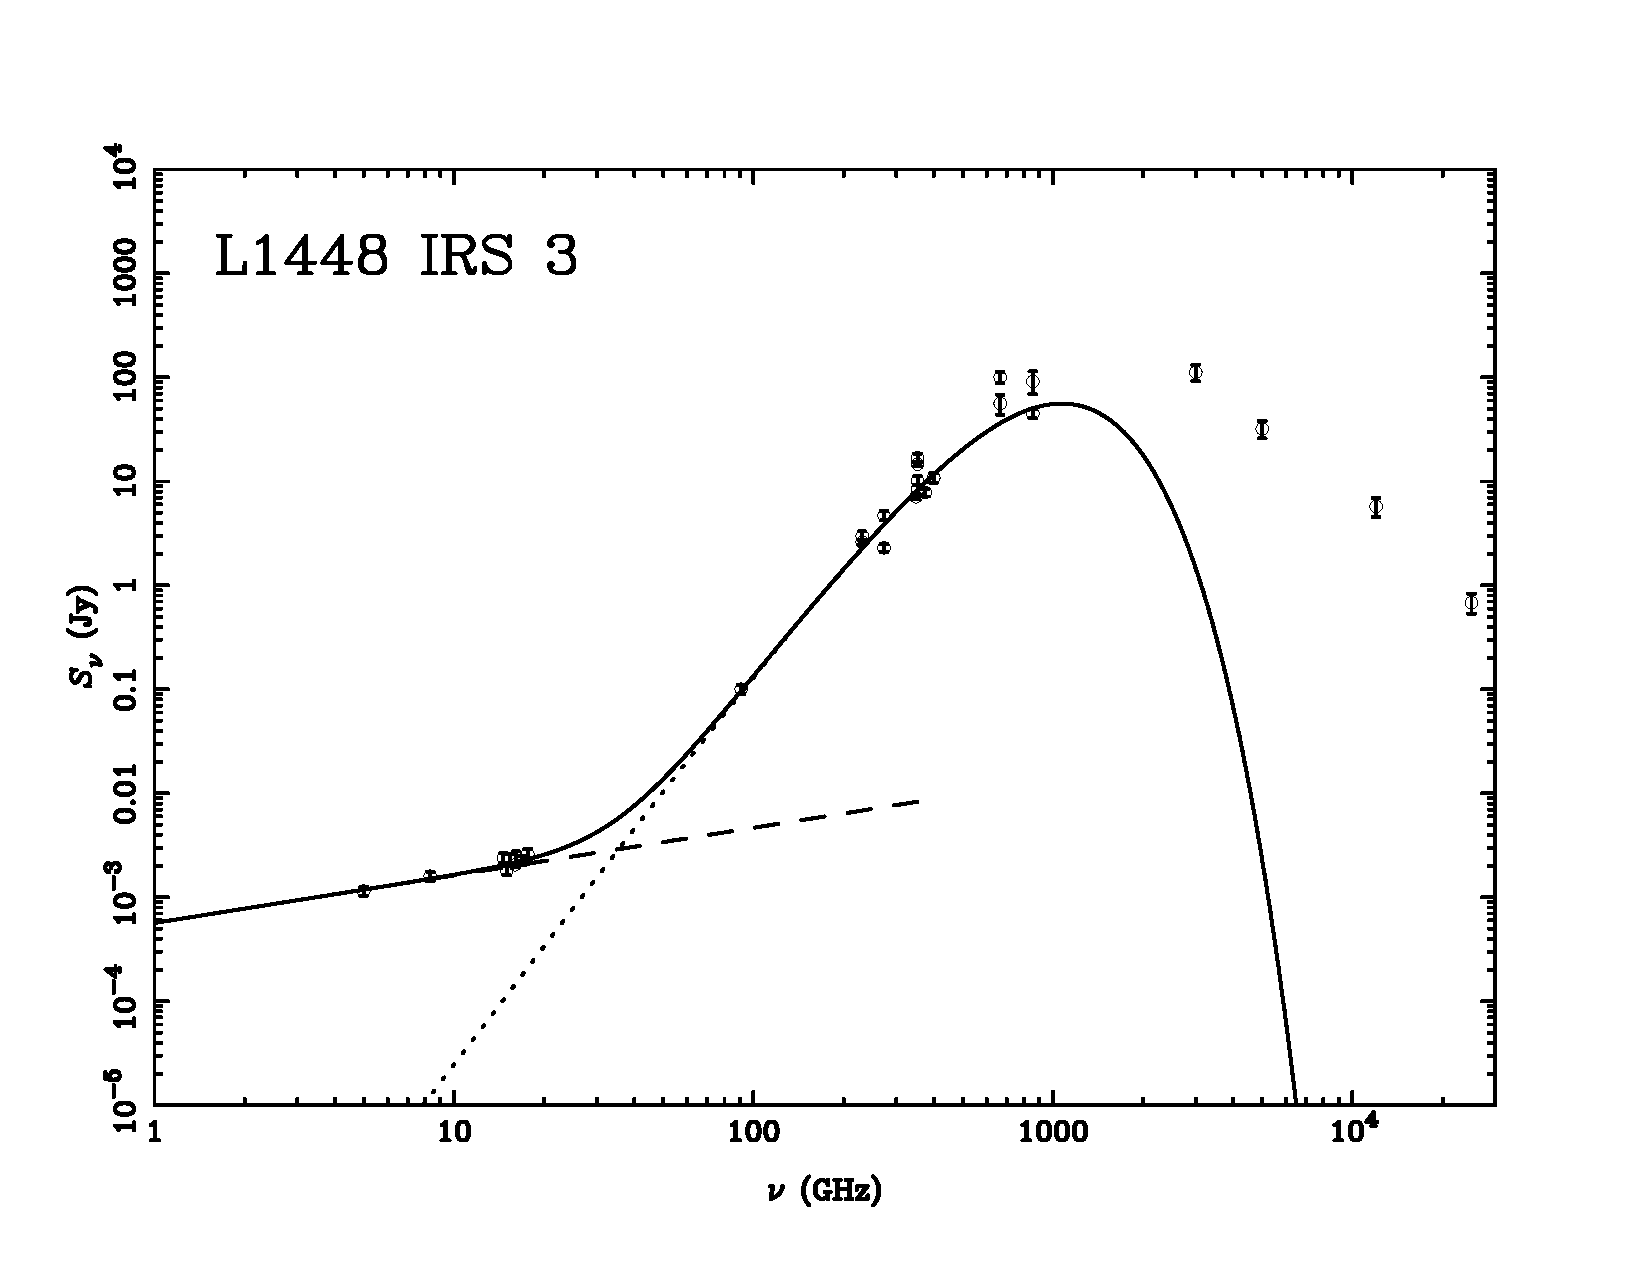
\includegraphics[width=0.65\textwidth]{plots/L1448.pdf}
\label{default}
\end{center}
\end{figure}

\clearpage



%%%%%
\begin{table}
\caption{HH~$7-11$}
\begin{center}
\begin{tabular}{llll}
\hline
 & $\nu$ & $S_\nu$ & Reference\\
 & (GHz) & (Jy) & \\
\hline
 & $5$ & $7.3\times10^{-4\dag}$ & \citet{1999ApJS..125..427R}\\
 & $8$ & $1.01\times10^{-3\dag}$ & \citet{1999ApJS..125..427R}\\
 & $14.62$ & $(3.43\pm0.20)\times10^{-3}$ & \citet{2012MNRAS.423.1089A}\\
 & $15.37$ & $(3.10\pm0.18)\times10^{-3}$ & \citet{2012MNRAS.423.1089A}\\
 & $16.12$ & $(3.91\pm0.22)\times10^{-3}$ & \citet{2012MNRAS.423.1089A}\\
 & $16.87$ & $(3.43\pm0.19)\times10^{-3}$ & \citet{2012MNRAS.423.1089A}\\
 & $17.62$ & $(3.83\pm0.24)\times10^{-3}$ & \citet{2012MNRAS.423.1089A}\\
 & $43$ & $(1.08\pm0.06)\times10^{-2}$ & \citet{2004ApJ...605L.137A}\\
 & $100$ & $(7.89\pm0.79)\times10^{-2}$ & \citet{2009ApJ...691.1729C}\\
 & $273$ & $4.46^{\dag}$ & \citet{2006ApJ...638..293E}\\
 & $353$ & $10.3^{\dag}$ & \citet{2008ApJS..175..277D}\\
 & $353$ & $12.7^{\dag}$ & \citet{2007AA...468.1009H}\\
 & $353$ & $14.9\pm1.2$ & \citet{2000ApJ...530..851C}\\
 & $400$ & $21.5\pm2.8$ & \citet{2000ApJ...530..851C}\\
 & $666$ & $119\pm24$ & \citet{2000ApJ...530..851C}\\
 & $666$ & $159.9^{\dag}$ & \citet{2007AA...468.1009H}\\
 & $857$ & $203\pm61$ & \citet{2000ApJ...530..851C}\\
 & $3\times10^{3}$ & $381\pm23$ & \textit{IRAS}\\
 & $5\times10^{3}$ & $204\pm20$ & \textit{IRAS}\\
 & $1.2\times10^{4}$ & $46.5\pm2.8$ & \textit{IRAS}\\
 & $2.5\times10^{4}$ & $13.6\pm3.7$ & \textit{IRAS}\\
\end{tabular}
\end{center}
\label{default}
\end{table}%

\begin{figure}[htbp]
\begin{center}
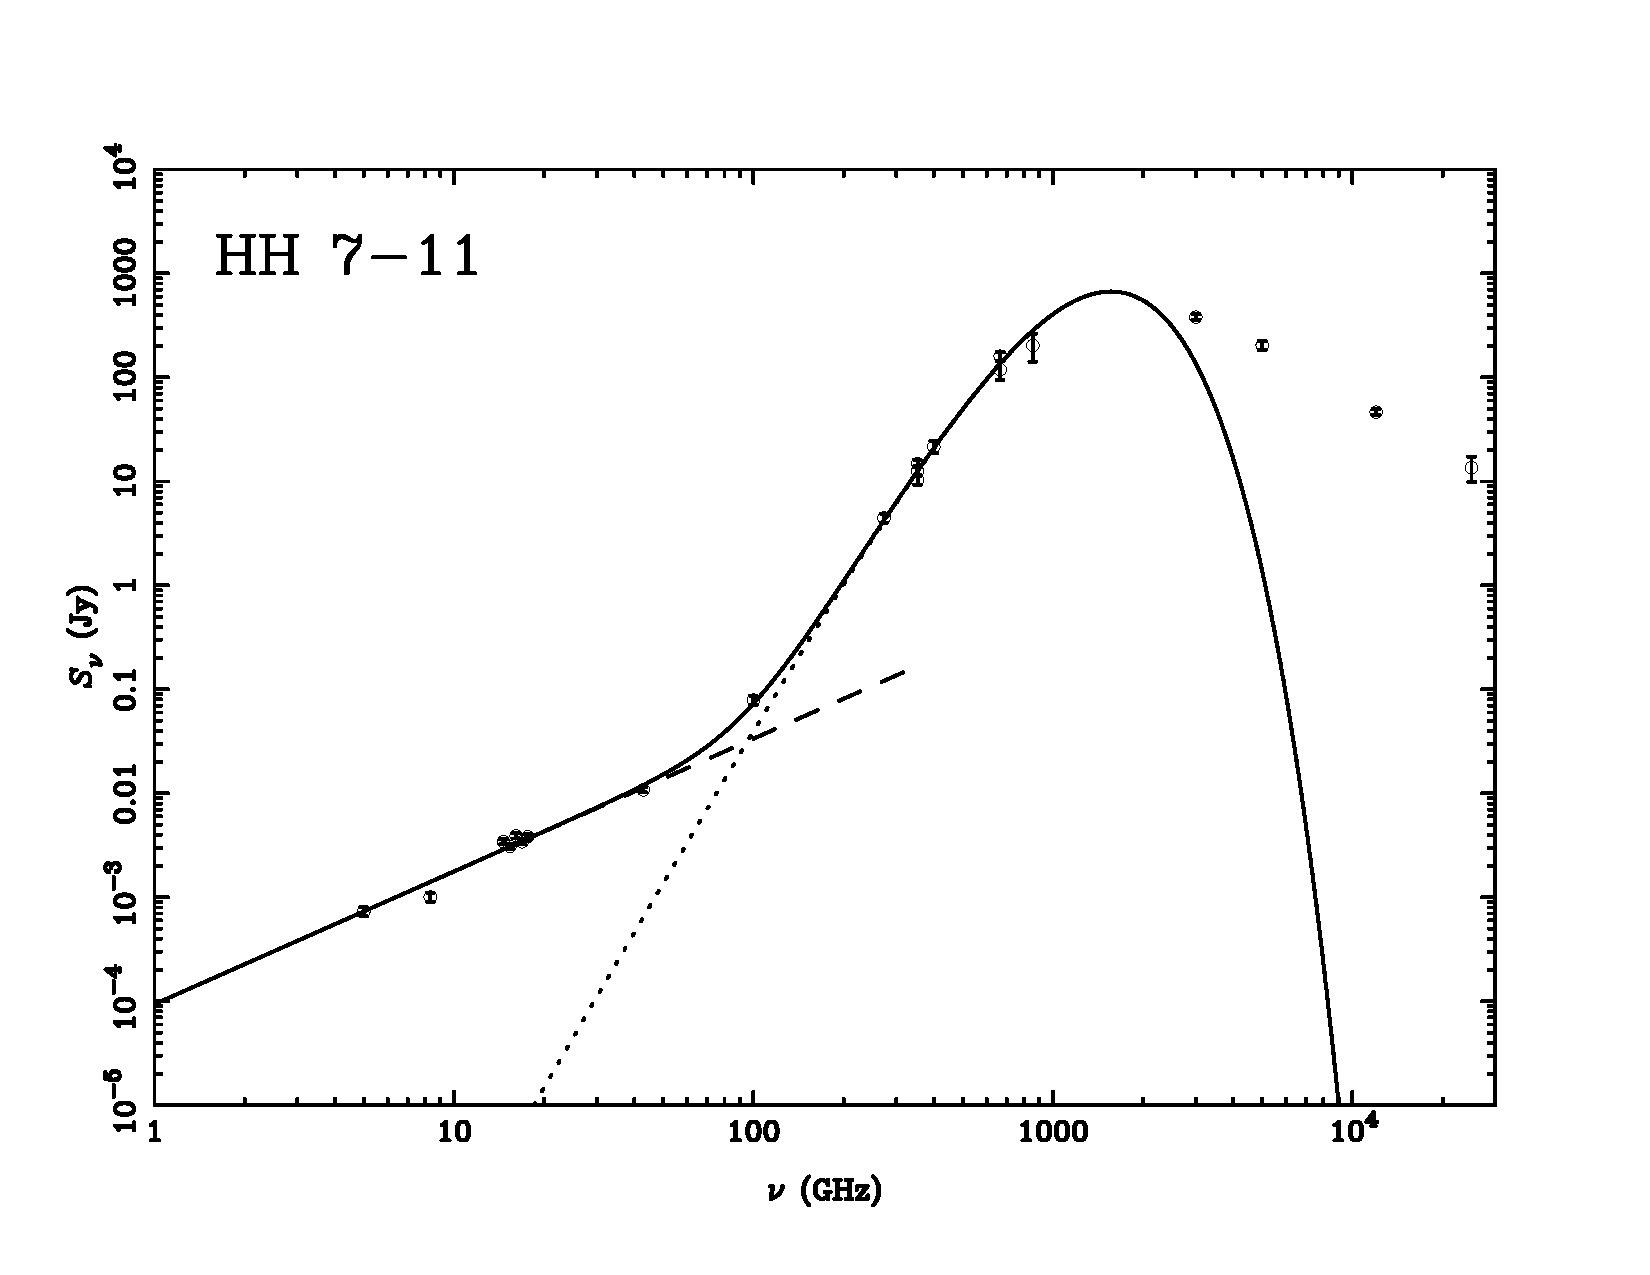
\includegraphics[width=0.65\textwidth]{plots/HH7-11.pdf}
\label{default}
\end{center}
\end{figure}

\clearpage




%%%%%
\begin{table}
\caption{L$1551$~IRS~$5$}
\begin{center}
\begin{tabular}{llll}
\hline
 & $\nu$ & $S_\nu$ & Reference\\
 & (GHz) & (Jy) & \\
\hline
 & $1.5$ & $2.28\times10^{-3\dag}$ & \citet{1985ApJ...289L...5B}\\
 & $1.5$ & $(2.8\pm0.9)\times10^{-3}$ & \citet{1985ApJ...290..587S}\\
 & $1.7$ & $4\times10^{-3\dag}$ & \citet{1989ApJ...337..712R}\\
 & $5$ & $4.2\times10^{-3\dag}$ & \citet{1987MNRAS.224..721D}\\
 & $5$ & $(3.5\pm0.5)\times10^{-3}$ & \citet{1982ApJ...253..707C}\\
 & $5$ & $3\times10^{-3\dag}$ & \citet{1984ApJ...282..699B}\\
 & $5$ & $4.69\times10^{-3\dag}$ & \citet{1985ApJ...289L...5B}\\
 & $5$ & $(4.3\pm0.5)\times10^{-3}$ & \citet{1985ApJ...290..587S}\\
 & $5$ & $(5\pm0.5)\times10^{-3}$ & \citet{1987ApJ...320..364E}\\
 & $5$ & $(4.1\pm0.4)\times10^{-3}$ & \citet{1990ApJ...355..635K}\\
 & $8$ & $(4.7\pm0.5)\times10^{-3}$ & \citet{1990ApJ...355..635K}\\
 & $14.62$ & $(4.74\pm0.25)\times10^{-3}$ & \citet{2012MNRAS.423.1089A}\\
 & $15$ & $2.25\times10^{-3\dag}$ & \citet{1986ApJ...301L..25R}\\
 & $15$ & $4.59\times10^{-3\dag}$ & \citet{1985ApJ...289L...5B}\\
 & $15$ & $(4.9\pm0.5)\times10^{-3}$ & \citet{1990ApJ...355..635K}\\
 & $15$ & $(3.6\pm0.2)\times10^{-3}$ & \citet{2003ApJ...583..330R}\\
 & $15$ & $(2.8\pm0.2)\times10^{-3}$ & \citet{2003ApJ...583..330R}\\
 & $15$ & $(3.3\pm0.2)\times10^{-3}$ & \citet{2003ApJ...583..330R}\\
 & $15$ & $(2.7\pm0.2)\times10^{-3}$ & \citet{2003ApJ...583..330R}\\
 & $15.37$ & $(3.10\pm0.18)\times10^{-3}$ & \citet{2012MNRAS.423.1089A}\\
 & $16.12$ & $(3.91\pm0.22)\times10^{-3}$ & \citet{2012MNRAS.423.1089A}\\
 & $16.87$ & $(3.43\pm0.19)\times10^{-3}$ & \citet{2012MNRAS.423.1089A}\\
 & $17.62$ & $(3.83\pm0.24)\times10^{-3}$ & \citet{2012MNRAS.423.1089A}\\
 & $22.5$ & $(1.7\pm0.4)\times10^{-2}$ & \citet{1985ApJ...288..595T}\\
 & $22.5$ & $(7.3\pm1.5)\times10^{-3}$ & \citet{1990ApJ...355..635K}\\
 & $23.7$ & $(7\pm1.4)\times10^{-3}$ & \citet{1993ApJ...414..333G}\\
 & $88$ & $0.09\pm0.03$ & \citet{1990ApJ...355..635K}\\
 & $90$ & $0.12^{\dag}$ & \citet{1994AA...281..161A}\\
 & $98$ & $0.13\pm0.004$ & \citet{1991AJ....102.2054O}\\
 & $110$ & $0.13\pm0.03$ & \citet{1990ApJ...355..635K}\\
 & $112$ & $0.15^{\dag}$ & \citet{1989ApJ...345..257W}\\
 & $113$ & $0.17^{\dag}$ & \citet{1986BAAS...18..973K}\\
 & $230$ & $1.5^{\dag}$ & \citet{1991ApJ...379L..25C}\\
 & $230$ & $1.57\pm0.02$ & \citet{1993AA...273..221R}\\
 & $231$ & $3.4^{\dag}$ & \citet{2001AA...365..440M}\\
 & $240$ & $2.37\pm0.48$ & \citet{1990ApJ...355..635K}\\
 & $250$ & $1.72^{\dag}$ & \citet{1994AA...281..161A}\\
 & $300$ & $5.7\pm1.3$ & \citet{1990ApJ...355..635K}\\
 & $345$ & $6.36\pm0.06$ & \citet{1993AA...273..221R}\\
 & $353$ & $19.01^{\dag}$ & \citet{2008ApJS..175..277D}\\
 & $353$ & $12.1\pm1$ & \citet{2000ApJ...530..851C}\\
 & $400$ & $18.2\pm2.4$ & \citet{2000ApJ...530..851C}\\
 & $666$ & $94\pm19$ & \citet{2000ApJ...530..851C}\\
 & $857$ & $164\pm49$ & \citet{2000ApJ...530..851C}\\
 & $3\times10^{3}$ & $458^{\dag}$ & \citet{1993AA...273..221R}\\
 & $5\times10^{3}$ & $373^{\dag}$ & \citet{1993AA...273..221R}\\
 & $1.2\times10^{4}$ & $106^{\dag}$ & \citet{1993AA...273..221R}\\
 & $2.5\times10^{4}$ & $10^{\dag}$ & \citet{1993AA...273..221R}\\
\end{tabular}
\end{center}
\label{default}
\end{table}%

\clearpage
\begin{figure}[htbp]
\begin{center}
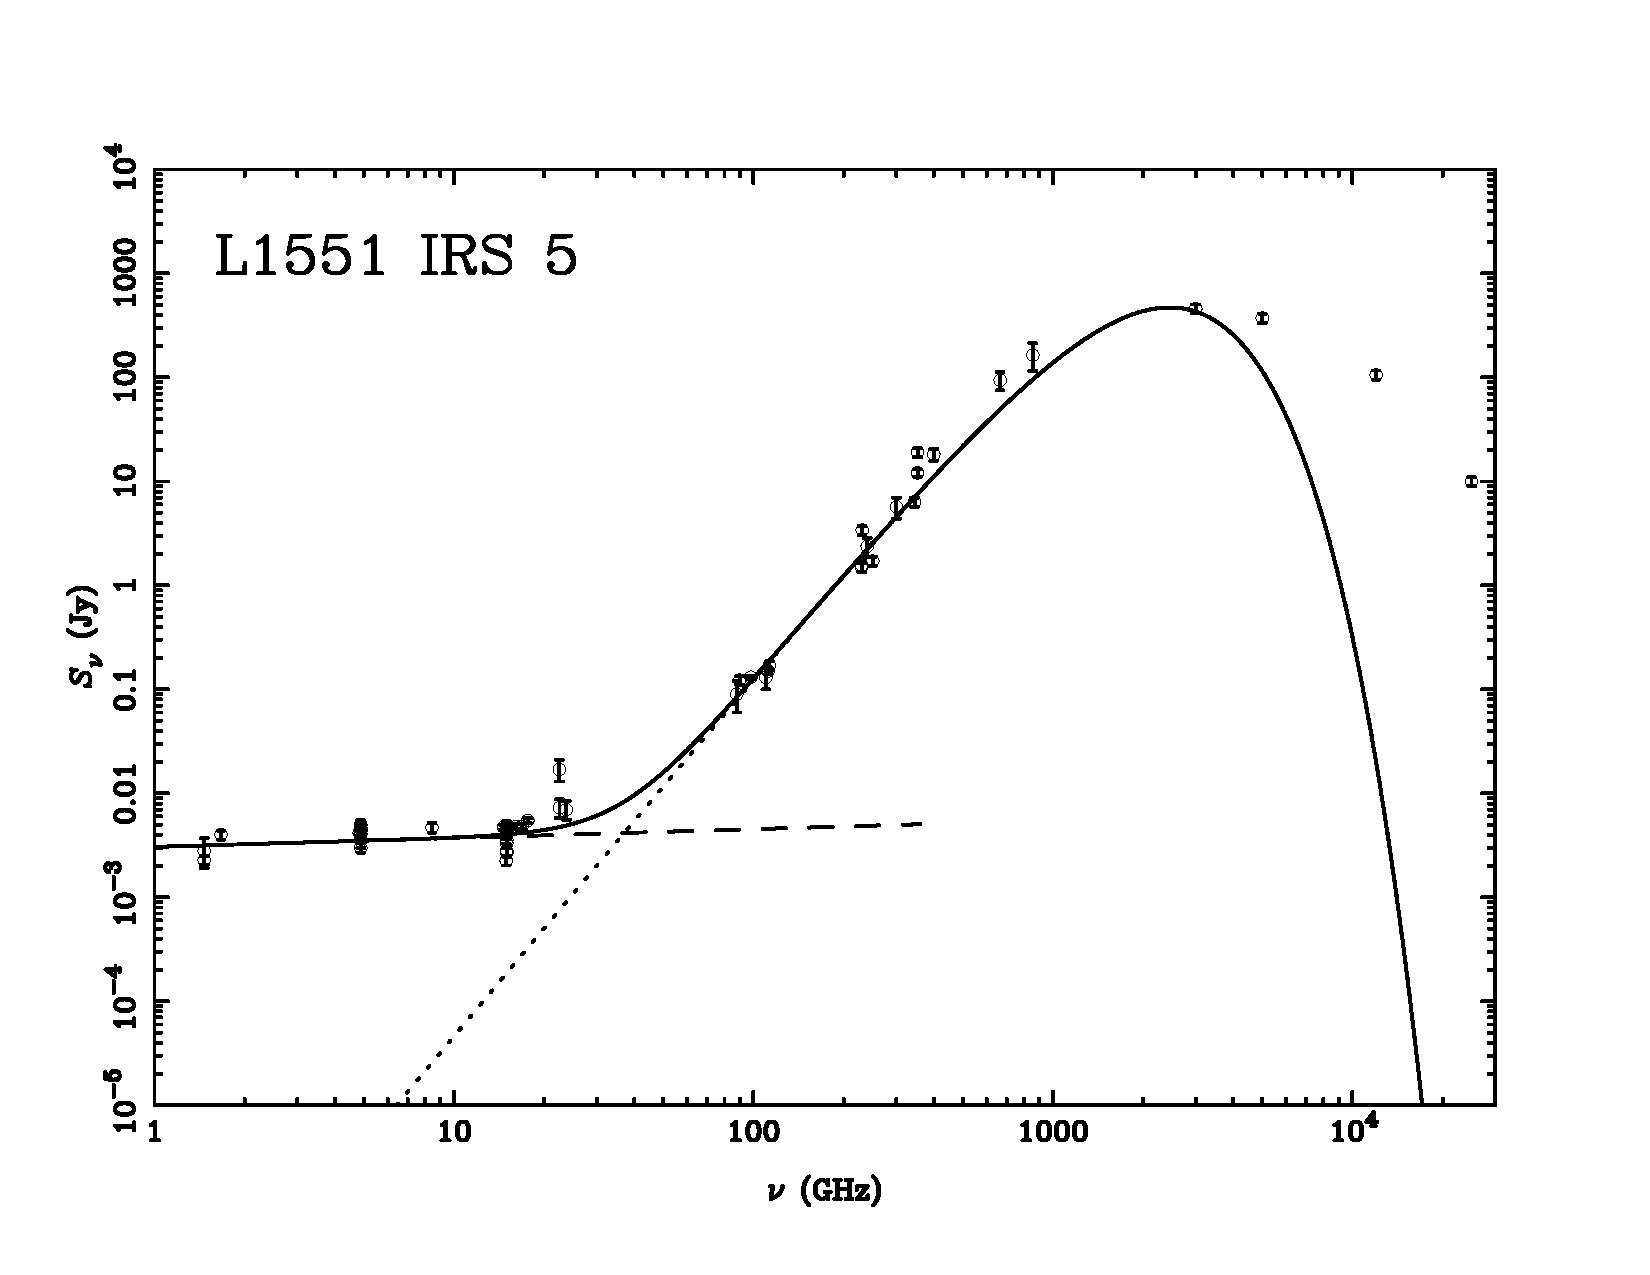
\includegraphics[width=0.65\textwidth]{plots/L1551.pdf}
\label{default}
\end{center}
\end{figure}

\clearpage



%%%%%
\begin{table}
\caption{L$1527$}
\begin{center}
\begin{tabular}{llll}
\hline
 & $\nu$ & $S_\nu$ & Reference\\
 & (GHz) & (Jy) & \\
\hline
 & $5$ & $(6.8\pm0.4)\times10^{-4}$ & \citet{2011ApJ...739L...7M}\\
 & $8.5$ & $(8.10\pm0.3)\times10^{-4}$ & \citet{2011ApJ...739L...7M}\\
 & $14.62$ & $(1.04\pm0.11)\times10^{-3}$ & \citet{2012MNRAS.423.1089A}\\
 & $15.37$ & $(1.04\pm0.14)\times10^{-3}$ & \citet{2012MNRAS.423.1089A}\\
 & $16$ & $(0.9\pm0.03)\times10^{-3}$ & \citet{2012MNRAS.420.3334S}\\
 & $16.12$ & $(1.12\pm0.13)\times10^{-3}$ & \citet{2012MNRAS.423.1089A}\\
 & $16.87$ & $(1.20\pm0.16)\times10^{-3}$ & \citet{2012MNRAS.423.1089A}\\
 & $17.62$ & $(1.38\pm0.15)\times10^{-3}$ & \citet{2012MNRAS.423.1089A}\\
 & $22.5$ & $(1.4\pm0.1)\times10^{-3}$ & \citet{2011ApJ...739L...7M}\\
 & $43.3$ & $(4.4\pm0.6)\times10^{-3}$ & \citet{2011ApJ...739L...7M}\\
 & $111$ & $(4.7\pm0.56)\times10^{-2}$ & \citet{1997ApJ...475..211O}\\
 & $230$ & $0.35^{\dag}$ & \citet{2010AJ....139.2504G}\\
 & $353$ & $0.90\pm0.01$ & \citet{2010AJ....139.2504G}\\
 & $375$ & $0.50^{\dag}$ & \citet{2010AJ....139.2504G}\\
 & $666$ & $2.85\pm0.22$ & \citet{2010AJ....139.2504G}\\
 & $666$ & $3.21^{\dag}$ & \citet{2010AJ....139.2504G}\\
 & $857$ & $12^{\dag}$ & \citet{2010AJ....139.2504G}\\
 & $1.87\times10^{3}$ & $68.8^{\dag}$ & \citet{2010AJ....139.2504G}\\
 & $3\times10^{3}$ & $71.3^{\dag}$ & \citet{2010AJ....139.2504G}\\
 & $3\times10^{3}$ & $72^{\dag}$ & \citet{2010AJ....139.2504G}\\
 & $5\times10^{3}$ & $17.4^{\dag}$ & \citet{2010AJ....139.2504G}\\
 & $5\times10^{3}$ & $18^{\dag}$ & \citet{2010AJ....139.2504G}\\
\end{tabular}
\end{center}
\label{default}
\end{table}%

\begin{figure}[htbp]
\begin{center}
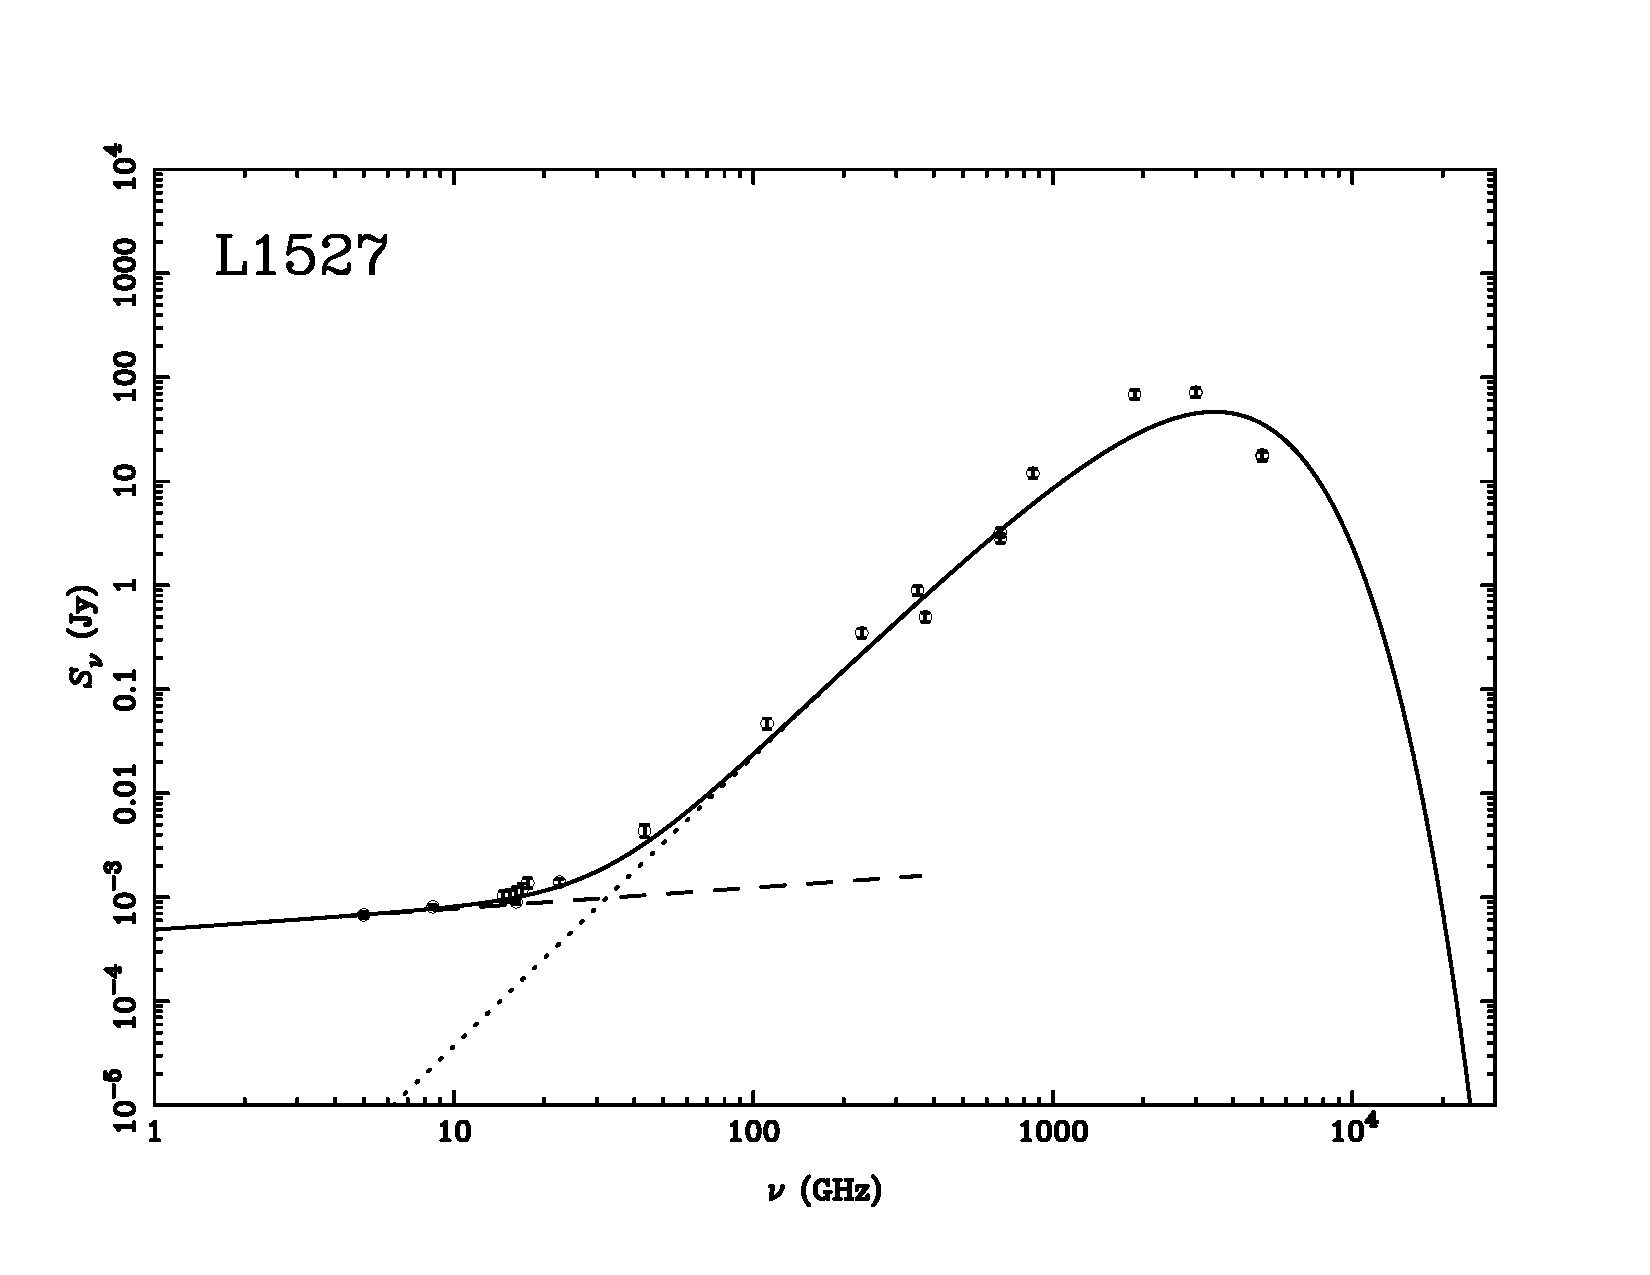
\includegraphics[width=0.65\textwidth]{plots/L1527.pdf}
\label{default}
\end{center}
\end{figure}

\clearpage



%%%%%
\begin{table}
\caption{HH~$1-2$~MMS~$1$}
\begin{center}
\begin{tabular}{llll}
\hline
 & $\nu$ & $S_\nu$ & Reference\\
 & (GHz) & (Jy) & \\
\hline
 & $1.5$ & $(6\pm2)\times10^{-4}$ & \citet{1985ApJ...293L..35P}\\
 & $1.5$ & $8.6\times10^{-4\dag}$ & \citet{1990ApJ...352..645R}\\
 & $5$ & $(1.19\pm1.6)\times10^{-3}$ & \citet{1990ApJ...362..274M}\\
 & $5$ & $(1.2\pm0.04)\times10^{-3}$ & \citet{1985ApJ...293L..35P}\\
 & $5$ & $1.17\times10^{-3\dag}$ & \citet{1990ApJ...352..645R}\\
 & $14.62$ & $(1.30\pm0.28)\times10^{-3}$ & \citet{2012MNRAS.423.1089A}\\
 & $15$ & $(1.54\pm0.18)\times10^{-3}$ & \citet{1985ApJ...293L..35P}\\
 & $15$ & $1.75\times10^{-3\dag}$ & \citet{1990ApJ...352..645R}\\
 & $15.37$ & $(1.53\pm0.30)\times10^{-3}$ & \citet{2012MNRAS.423.1089A}\\
 & $16.12$ & $(1.34\pm0.18)\times10^{-3}$ & \citet{2012MNRAS.423.1089A}\\
 & $16.87$ & $(1.33\pm0.14)\times10^{-3}$ & \citet{2012MNRAS.423.1089A}\\
 & $230$ & $0.65\pm0.02$ & \citet{1993AA...273..221R}\\
 & $273$ & $0.92\pm0.03$ & \citet{1998MNRAS.301.1049D}\\
 & $345$ & $1.67\pm0.02$ & \citet{1993AA...273..221R}\\
 & $353$ & $9.44^{\dag}$ & \citet{2008ApJS..175..277D}\\
 & $354$ & $1.2\pm0.24$ & \citet{2010AA...518L.122F}\\
 & $375$ & $2.65\pm0.03$ & \citet{1998MNRAS.301.1049D}\\
 & $666$ & $18.9\pm0.35$ & \citet{1998MNRAS.301.1049D}\\
 & $857$ & $33.95\pm0.29$ & \citet{1998MNRAS.301.1049D}\\
 & $857$ & $28\pm11.2$ & \citet{2010AA...518L.122F}\\
 & $1.88\times10^{3}$ & $75.7\pm15.14$ & \citet{2010AA...518L.122F}\\
 & $4.29\times10^{3}$ & $26.6\pm2.66$ & \citet{2010AA...518L.122F}\\
\end{tabular}
\end{center}
\label{default}
\end{table}%

\begin{figure}[htbp]
\begin{center}
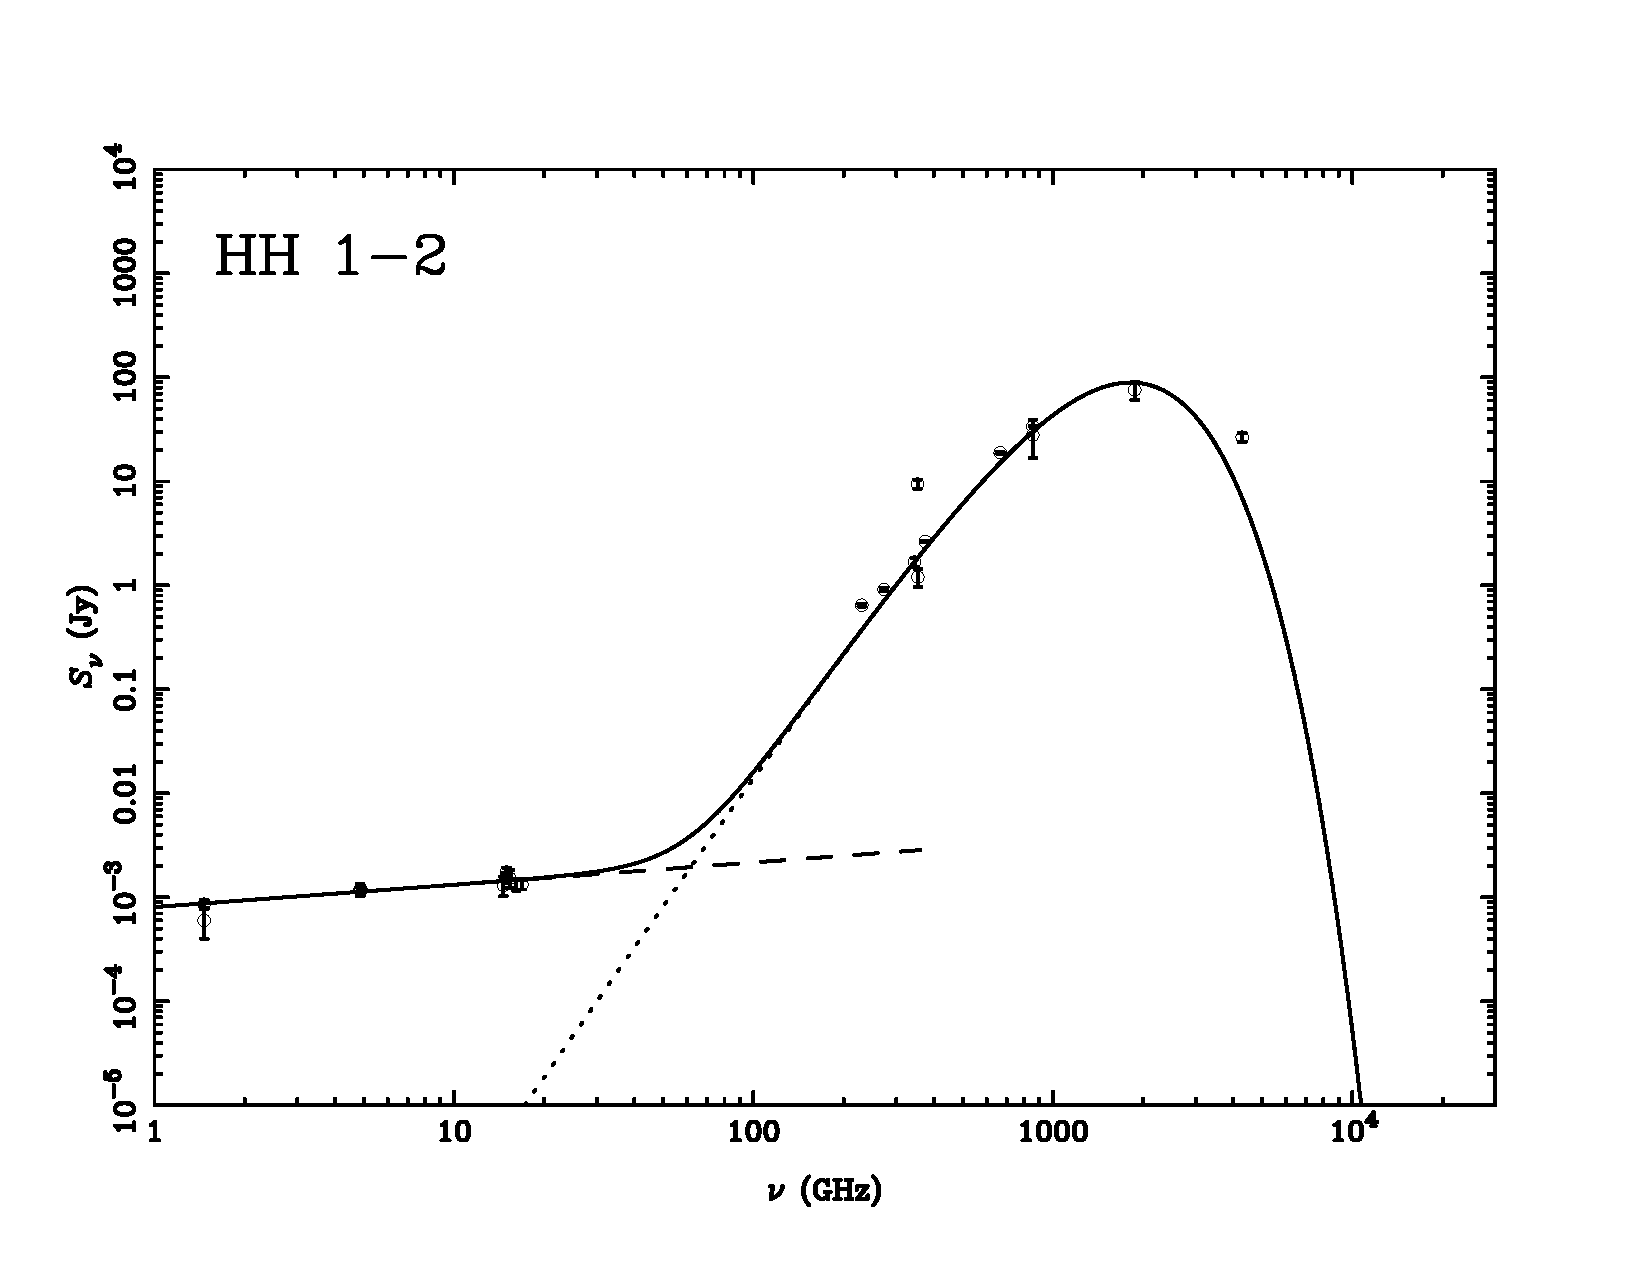
\includegraphics[width=0.65\textwidth]{plots/HH1-2.pdf}
\label{default}
\end{center}
\end{figure}

\clearpage



%%%%%
\begin{table}
\caption{HH~$26$~IR}
\begin{center}
\begin{tabular}{llll}
\hline
 & $\nu$ & $S_\nu$ & Reference\\
 & (GHz) & (Jy) & \\
\hline
 & $8$ & $(3.8\pm0.6)\times10^{-4}$ & \citet{1998AJ....116.2953A}\\
 & $8$ & $(1.4\pm0.3)\times10^{-4}$ & \citet{1999MNRAS.304....1G}\\
 & $16.12$ & $(3.92\pm0.76)\times10^{-4}$ & \citet{2012MNRAS.423.1089A}\\
 & $231$ & $0.32^{\dag}$ & \citet{1999ApJ...527..856L}\\
 & $353$ & $0.97^{\dag}$ & \citet{2008ApJS..175..277D}\\
 & $353$ & $0.9\pm0.09$ & \citet{2007MNRAS.374.1413N}\\
 & $666$ & $1.4\pm0.28$ & \citet{2007MNRAS.374.1413N}\\
 & $857$ & $6.3^{\dag}$ & \citet{1999ApJ...527..856L}\\
 & $4.29\times10^{3}$ & $7.9^{\dag}$ & \citet{2008AA...479..503A}\\
 & $5\times10^{3}$ & $20.87^{\dag}$ & \citet{2008AA...479..503A}\\
 & $1.2\times10^{4}$ & $5.13^{\dag}$ & \citet{2008AA...479..503A}\\
 & $1.25\times10^{3}$ & $1.8^{\dag}$ & \citet{2008AA...479..503A}\\
 & $2.5\times10^{4}$ & $1.93^{\dag}$ & \citet{2008AA...479..503A}\\
\end{tabular}
\end{center}
\label{default}
\end{table}%

\begin{figure}[htbp]
\begin{center}
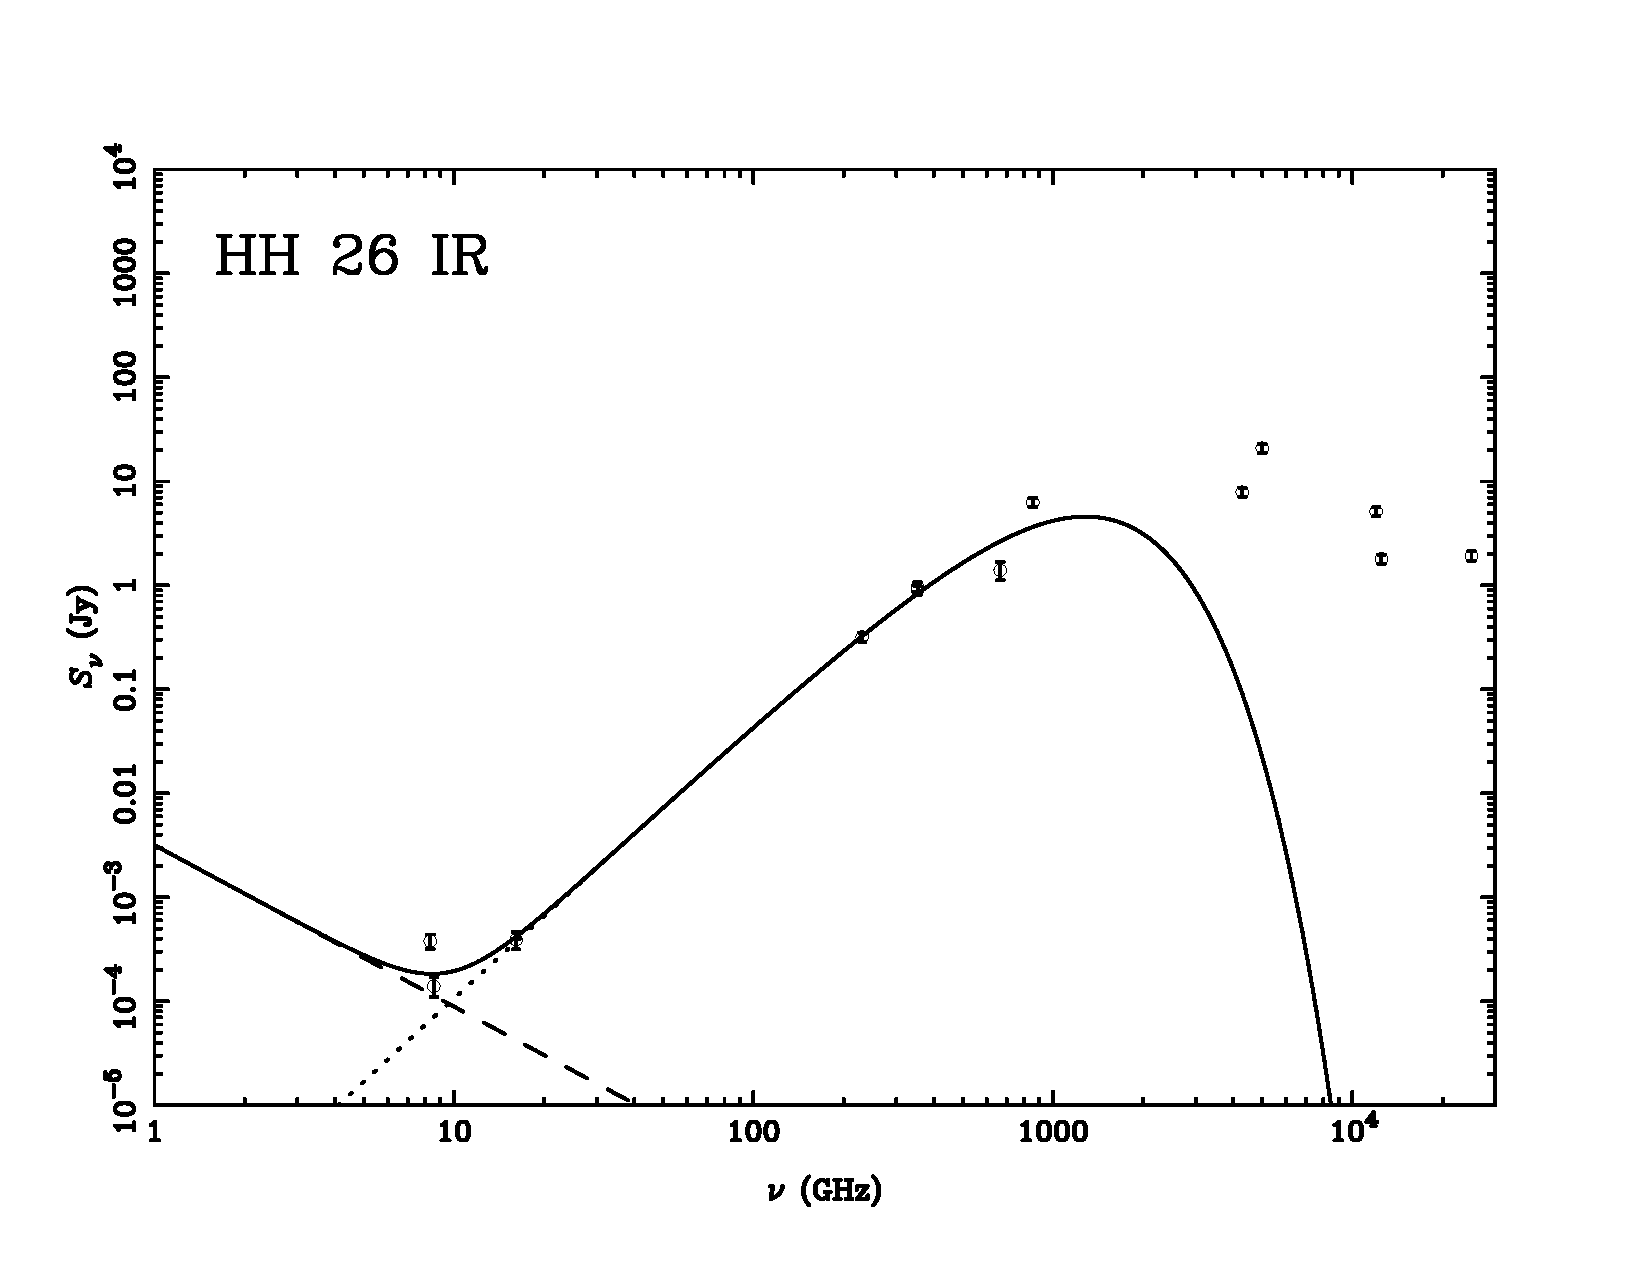
\includegraphics[width=0.65\textwidth]{plots/HH26IR.pdf}
\label{default}
\end{center}
\end{figure}

\clearpage



%%%%%
\begin{table}
\caption{HH~$111$}
\begin{center}
\begin{tabular}{llll}
\hline
 & $\nu$ & $S_\nu$ & Reference\\
 & (GHz) & (Jy) & \\
\hline
 & $5$ & $(8.3\pm0.9)\times10^{-4}$ & \citet{2008AJ....136.1852R}\\
 & $8$ & $(9.5\pm0.4)\times10^{-4}$ & \citet{1994AA...281..882R}\\
 & $14.62$ & $(3.11\pm0.53)\times10^{-3}$ & \citet{2012MNRAS.423.1089A}\\
 & $15$ & $(2.3\pm0.32)\times10^{-3}$ & \citet{1994AA...281..882R}\\
 & $15.37$ & $(2.68\pm0.28)\times10^{-3}$ & \citet{2012MNRAS.423.1089A}\\
 & $16.12$ & $(2.39\pm0.26)\times10^{-3}$ & \citet{2012MNRAS.423.1089A}\\
 & $16.87$ & $(2.86\pm0.30)\times10^{-3}$ & \citet{2012MNRAS.423.1089A}\\
 & $17.62$ & $(2.51\pm0.34)\times10^{-3}$ & \citet{2012MNRAS.423.1089A}\\
 & $43$ & $(5.15\pm0.52)\times10^{-3}$ & \citet{2008AJ....136.1852R}\\
 & $110$ & $(4.6\pm0.46)\times10^{-2}$ & \citet{1993ApJ...408..239S}\\
 & $230$ & $0.49\pm0.02$ & \citet{1993AA...273..221R}\\
 & $230$ & $0.47\pm0.05$ & \citet{1989ApJ...345..257W}\\
 & $273$ & $0.75\pm0.01$ & \citet{1998MNRAS.301.1049D}\\
 & $285$ & $0.69^{\dag}$ & \citet{1993ApJ...408..239S}\\
 & $345$ & $1.39\pm0.03$ & \citet{1993AA...273..221R}\\
 & $353$ & $3.09^{\dag}$ & \citet{2008ApJS..175..277D}\\
 & $375$ & $1.8\pm0.02$ & \citet{1998MNRAS.301.1049D}\\
 & $666$ & $8.22\pm0.26$ & \citet{1998MNRAS.301.1049D}\\
 & $857$ & $14.2\pm0.9$ & \citet{1998MNRAS.301.1049D}\\
 & $3\times10^{3}$ & $71.1^{\dag}$ & \citet{1993AA...273..221R}\\
 & $5\times10^{3}$ & $43.5^{\dag}$ & \citet{1993AA...273..221R}\\
 & $1.2\times10^{4}$ & $6.8^{\dag}$ & \citet{1993AA...273..221R}\\
 & $2.5\times10^{4}$ & $0.3^{\dag}$ & \citet{1993AA...273..221R}\\
\end{tabular}
\end{center}
\label{default}
\end{table}%

\begin{figure}[htbp]
\begin{center}
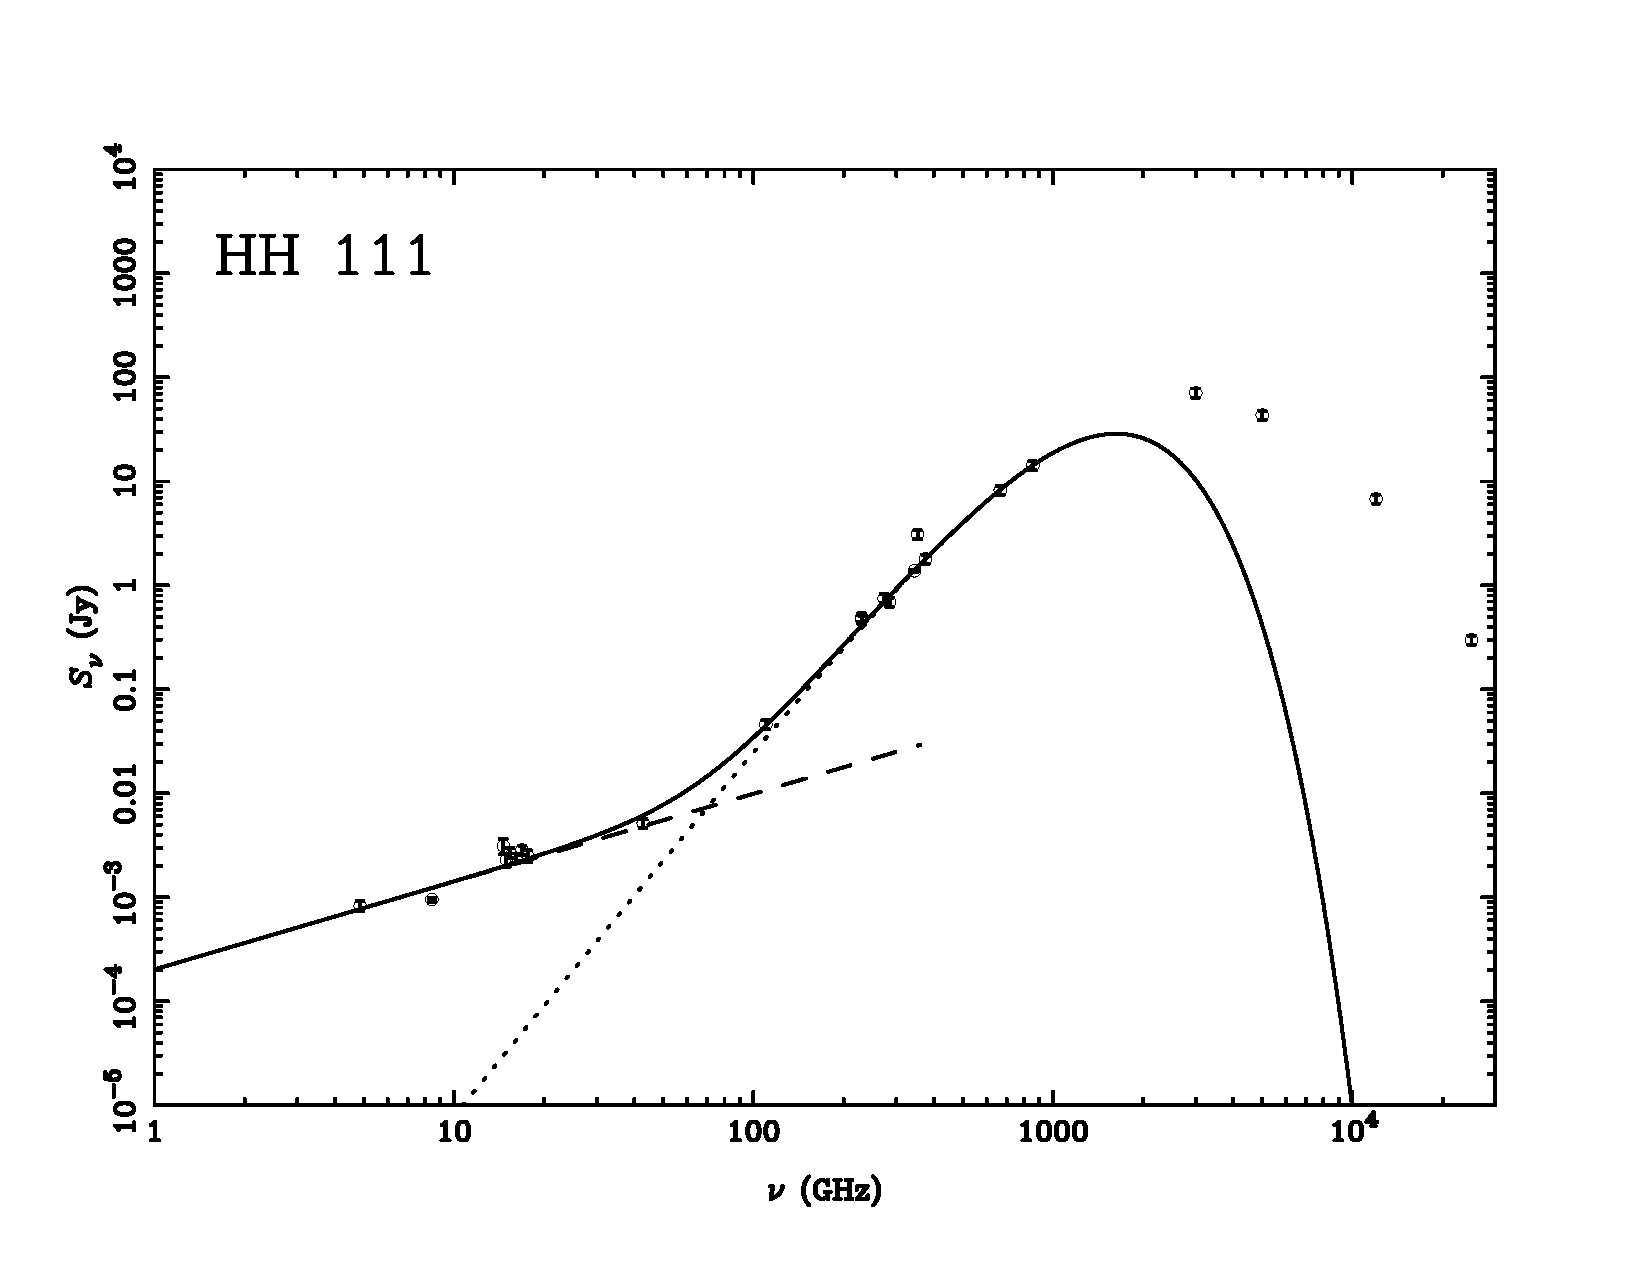
\includegraphics[width=0.65\textwidth]{plots/HH111.pdf}
\label{default}
\end{center}
\end{figure}

\clearpage



%%%%%
\begin{table}
\caption{NGC~$2264$~G}
\begin{center}
\begin{tabular}{llll}
\hline
 & $\nu$ & $S_\nu$ & Reference\\
 & (GHz) & (Jy) & \\
\hline
 & $1.5$ & $(8\pm2)\times10^{-4}$ & \citet{1989RMxAA..17..115R}\\
 & $5$ & $(1.9\pm0.2)\times10^{-3}$ & \citet{1989RMxAA..17..115R}\\
 & $5$ & $6.7\times10^{-4\dag}$ & \citet{1994ApJ...436..749G}\\
 & $8$ & $5.5\times10^{-4\dag}$ & \citet{1994ApJ...436..749G}\\
 & $16.12$ & $(2.96\pm2.16)\times10^{-4}$ & \citet{2012MNRAS.423.1089A}\\
 & $273$ & $0.25\pm0.04$ & \citet{1995MNRAS.273L..25W}\\
 & $353$ & $0.71^{\dag}$ & \citet{2008ApJS..175..277D}\\
 & $375$ & $0.7\pm0.04$ & \citet{1995MNRAS.273L..25W}\\
 & $666$ & $3.9\pm0.1$ & \citet{1995MNRAS.273L..25W}\\
 & $857$ & $7.1\pm0.28$ & \citet{1995MNRAS.273L..25W}\\
 & $3\times10^{3}$ & $17\pm3$ & \citet{1995MNRAS.273L..25W}\\
 & $5\times10^{3}$ & $6\pm1$ & \citet{1995MNRAS.273L..25W}\\
\end{tabular}
\end{center}
\label{default}
\end{table}%

\begin{figure}[htbp]
\begin{center}
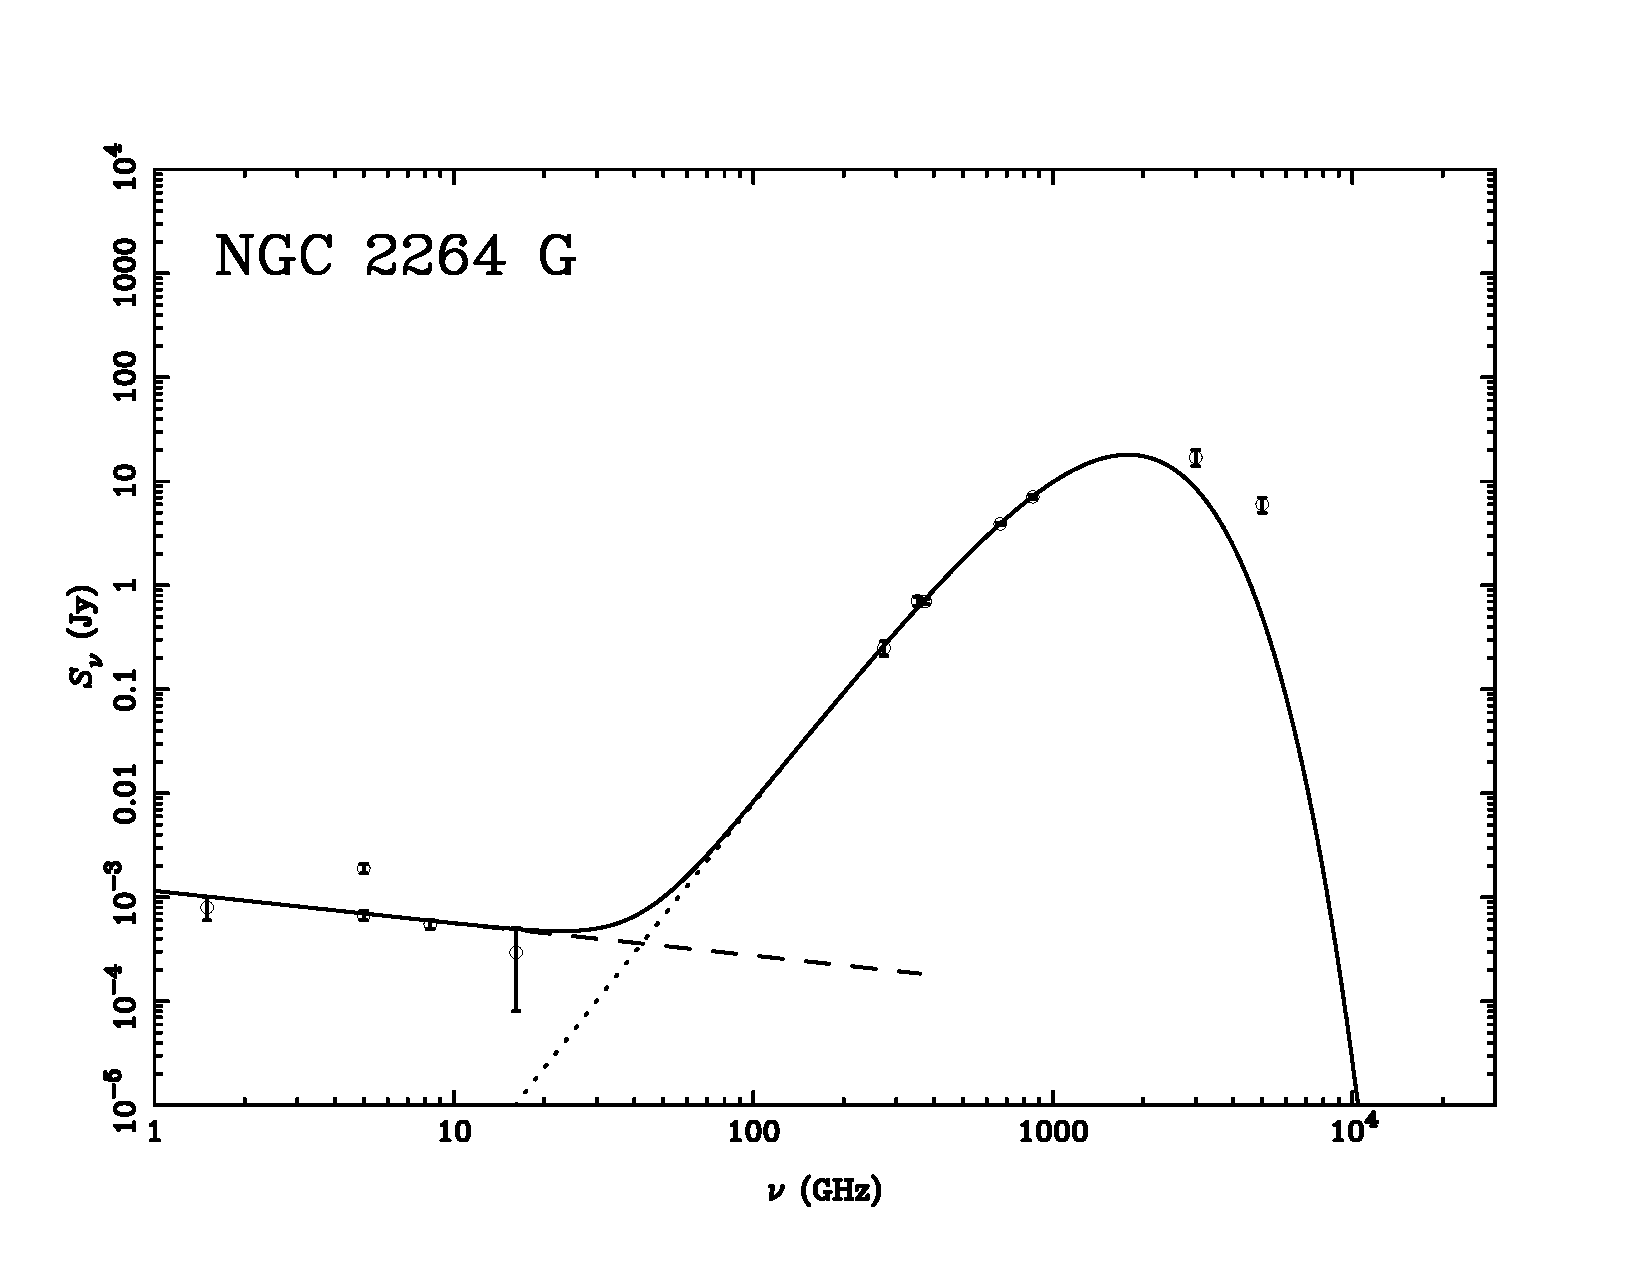
\includegraphics[width=0.65\textwidth]{plots/NGC2264.pdf}
\label{default}
\end{center}
\end{figure}

\clearpage



%%%%%
\begin{table}
\caption{Serpens~SMM~$1$}
\begin{center}
\begin{tabular}{llll}
\hline
 & $\nu$ & $S_\nu$ & Reference\\
 & (GHz) & (Jy) & \\
\hline
 & $1.5$ & $(4.5\pm0.5)\times10^{-3}$ & \citet{1998AJ....115.1693C}\\
 & $1.5$ & $(9.5\pm0.49)\times10^{-3}$ & \citet{1993ApJ...415..191C}\\
 & $5$ & $(9.5\pm0.8)\times10^{-3}$ & \citet{1986ApJ...303..683S}\\
 & $5$ & $(7.9\pm0.48)\times10^{-3}$ & \citet{1989ApJ...346L..85R}\\
 & $5$ & $(7.6\pm0.3)\times10^{-3}$ & \citet{1993ApJ...415..191C}\\
 & $5$ & $2.2\times10^{-3\dag}$ & \citet{1994ApJ...424..222M}\\
 & $8$ & $(7.5\pm0.17)\times10^{-3}$ & \citet{1993ApJ...415..191C}\\
 & $8$ & $7.54\times10^{-3\dag}$ & \citet{2005AJ....130..643E}\\
 & $14.62$ & $(8.21\pm0.77)\times10^{-3}$ & \citet{2012MNRAS.423.1089A}\\
 & $15$ & $(1\pm0.3)\times10^{-2}$ & \citet{1986ApJ...303..683S}\\
 & $15$ & $(8.3\pm0.3)\times10^{-3}$ & \citet{1993ApJ...415..191C}\\
 & $15$ & $(6.2\pm0.0.44)\times10^{-3}$ & \citet{1989ApJ...346L..85R}\\
 & $15$ & $4.8\times10^{-3\dag}$ & \citet{1994ApJ...424..222M}\\
 & $15.37$ & $(7.66\pm0.55)\times10^{-3}$ & \citet{2012MNRAS.423.1089A}\\
 & $16$ & $(4.74\pm0.24)\times10^{-3}$ & \citet{2012MNRAS.420.1019A}\\
 & $16.12$ & $(7.04\pm0.43)\times10^{-3}$ & \citet{2012MNRAS.423.1089A}\\
 & $16.87$ & $(6.77\pm0.44)\times10^{-3}$ & \citet{2012MNRAS.423.1089A}\\
 & $17.62$ & $(7.30\pm0.54)\times10^{-3}$ & \citet{2012MNRAS.423.1089A}\\
 & $23$ & $5.3\times10^{-3\dag}$ & \citet{1994ApJ...424..222M}\\
 & $43$ & $(1.42\pm0.04)\times10^{-2}$ & \citet{2009ApJ...705.1730C}\\
 & $88$ & $0.2^{\dag}$ & \citet{1999ApJ...513..350H}\\
 & $94$ & $0.2^{\dag}$ & \citet{1999ApJ...513..350H}\\
 & $97$ & $0.14^{\dag}$ & \citet{1994ApJ...424..222M}\\
 & $111$ & $0.41^{\dag}$ & \citet{1999ApJ...513..350H}\\
 & $214$ & $2.65^{\dag}$ & \citet{1999ApJ...513..350H}\\
 & $240$ & $2.3^{\dag}$ & \citet{1994ApJ...424..222M}\\
 & $273$ & $3.47\pm0.1$ & \citet{1993AA...275..195C}\\
 & $353$ & $15.23{\dag}$ & \citet{2008ApJS..175..277D}\\
 & $353$ & $6.1^{\dag}$ & \citet{1999MNRAS.309..141D}\\
 & $666$ & $35.7^{\dag}$ & \citet{1999MNRAS.309..141D}\\
 & $1.88\times10^{3}$ & $430^{\dag}$ & \citet{1994ApJ...424..222M}\\
 & $3\times10^{3}$ & $380^{\dag}$ & \citet{1994ApJ...424..222M}\\
 & $5\times10^{3}$ & $152.92^{\dag}$ & \citet{1994ApJ...424..222M}\\
 & $6\times10^{3}$ & $88.6^{\dag}$ & \citet{1994ApJ...424..222M}\\
 & $1.2\times10^{4}$ & $3.17^{\dag}$ & \citet{1994ApJ...424..222M}\\
 & $1.5\times10^{4}$ & $2.6^{\dag}$ & \citet{1994ApJ...424..222M}\\
 & $2.5\times10^{4}$ & $0.25^{\dag}$ & \citet{1994ApJ...424..222M}\\
\end{tabular}
\end{center}
\label{default}
\end{table}%

\clearpage
\begin{figure}[htbp]
\begin{center}
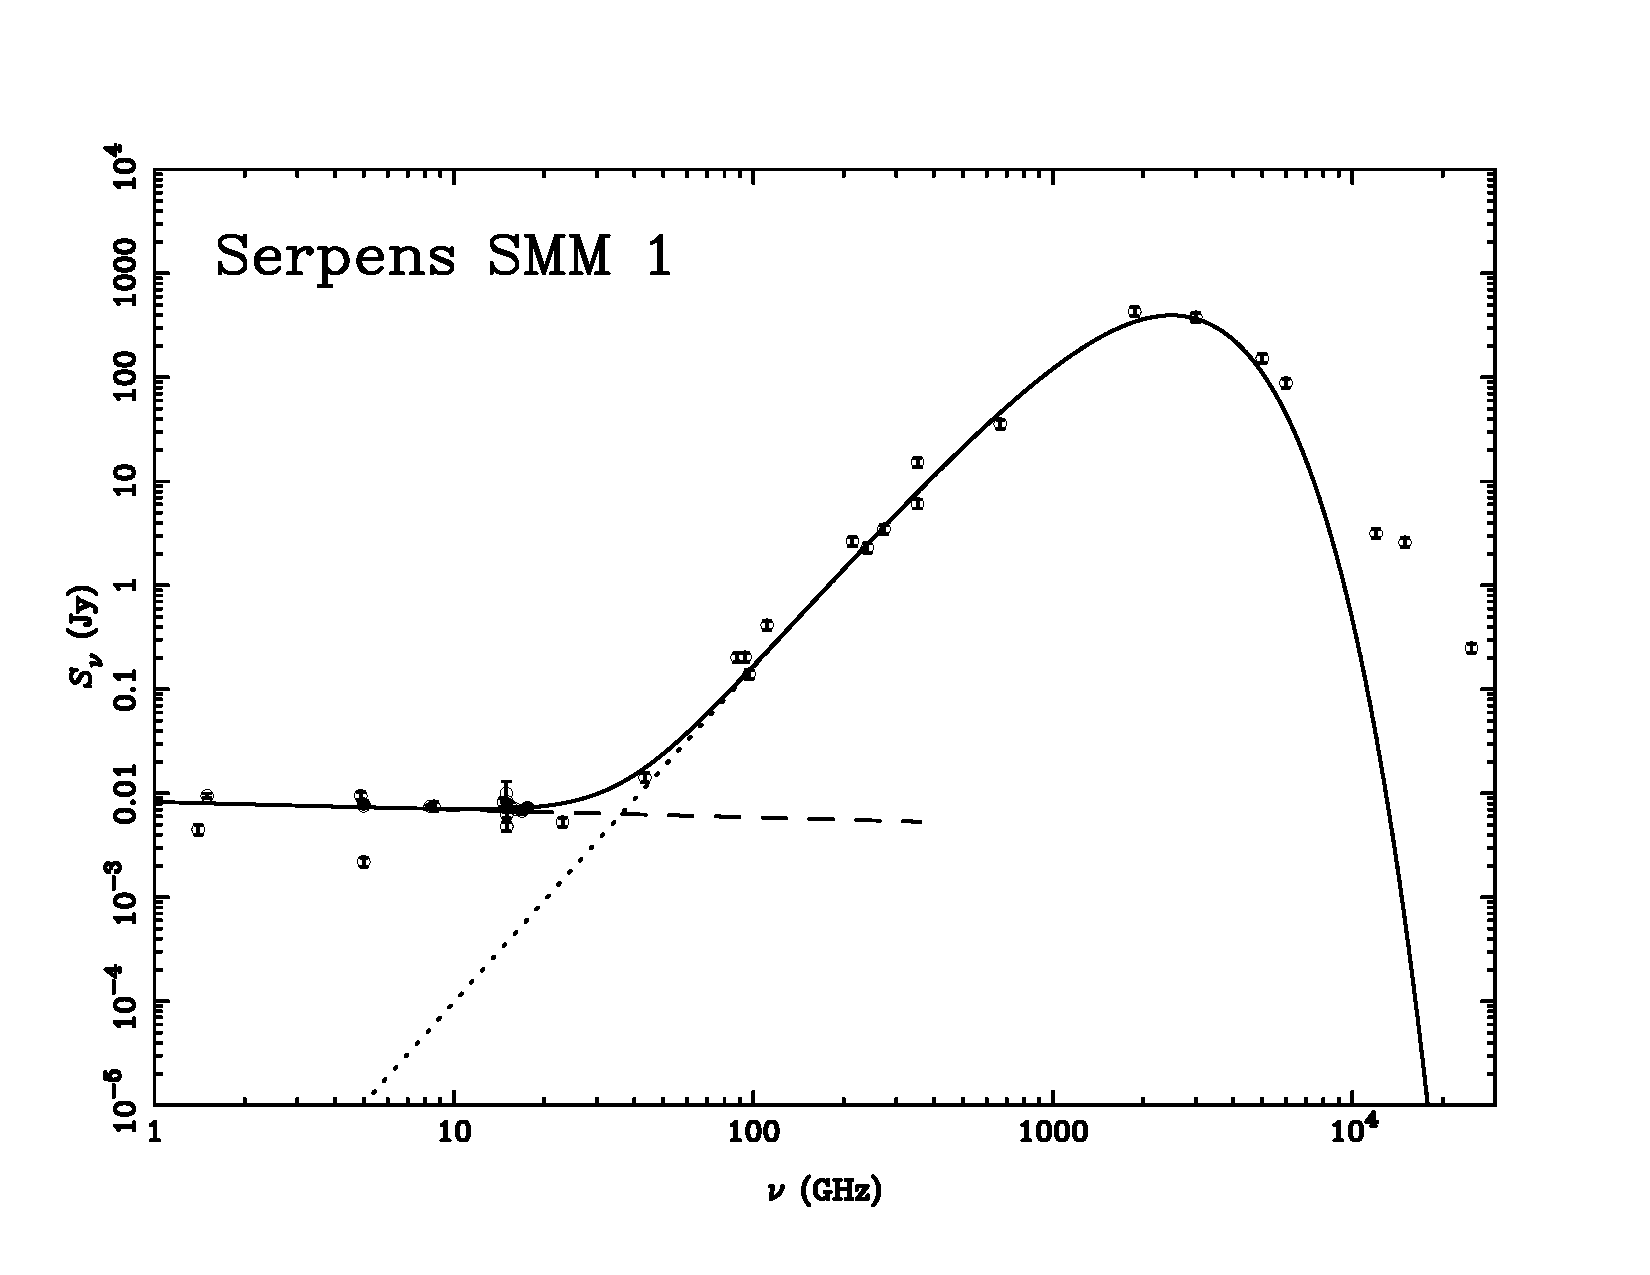
\includegraphics[width=0.65\textwidth]{plots/Serpens.pdf}
\label{default}
\end{center}
\end{figure}

\clearpage



%%%%%
\begin{table}
\caption{L$723$}
\begin{center}
\begin{tabular}{llll}
\hline
 & $\nu$ & $S_\nu$ & Reference\\
 & (GHz) & (Jy) & \\
\hline
 & $5$ & $7.5\times10^{-4\dag}$ & \citet{1996ApJ...473L.123A}\\
 & $8$ & $7.6\times10^{-4\dag}$ & \citet{1996ApJ...473L.123A}\\
 & $14.62$ & $(5.82\pm0.86)\times10^{-4}$ & \citet{2012MNRAS.423.1089A}\\
 & $15.37$ & $(5.16\pm0.64)\times10^{-4}$ & \citet{2012MNRAS.423.1089A}\\
 & $16.12$ & $(6.53\pm0.78)\times10^{-4}$ & \citet{2012MNRAS.423.1089A}\\
 & $16.87$ & $(6.55\pm0.69)\times10^{-4}$ & \citet{2012MNRAS.423.1089A}\\
 & $17.62$ & $(5.22\pm1.00)\times10^{-4}$ & \citet{2012MNRAS.423.1089A}\\
 & $230$ & $0.37^{\dag}$ & \citet{2001AA...365..440M}\\
 & $230$ & $0.36\pm0.02$ & \citet{1993AA...273..221R}\\
 & $300$ & $1\pm0.5$ & \citet{1993AA...273..221R}\\
 & $353$ & $1.79\pm0.11$ & \citet{2000ApJS..131..249S}\\
 & $353$ & $2.24^{\dag}$ & \citet{2008ApJS..175..277D}\\
 & $666$ & $8.5\pm2.1$ & \citet{2000ApJS..131..249S}\\
 & $750$ & $13\pm3$ & \citet{1993AA...273..221R}\\
 & $857$ & $11.3\pm1.8$ & \citet{2007AJ....133.1560W}\\
 & $1.54\times10^{3}$ & $35\pm7$ & \citet{1993AA...273..221R}\\
 & $1.81\times10^{3}$ & $40\pm12$ & \citet{1993AA...273..221R}\\
 & $2.08\times10^{3}$ & $33\pm10$ & \citet{1993AA...273..221R}\\
 & $2.14\times10^{3}$ & $23\pm8$ & \citet{1993AA...273..221R}\\
 & $2.31\times10^{3}$ & $32\pm11$ & \citet{1993AA...273..221R}\\
 & $3\times10^{3}$ & $20.7\pm1.7$ & \citet{2000ApJS..131..249S}\\
 & $3.16\times10^{3}$ & $27\pm6$ & \citet{2000ApJS..131..249S}\\
 & $5\times10^{3}$ & $6.93\pm0.62$ & \citet{2000ApJS..131..249S}\\
 & $1.2\times10^{4}$ & $0.38\pm0.05$ & \citet{2000ApJS..131..249S}\\
 & $2.5\times10^{4}$ & $0.28\pm0.06$ & \citet{2000ApJS..131..249S}\\
\end{tabular}
\end{center}
\label{default}
\end{table}%

\begin{figure}[htbp]
\begin{center}
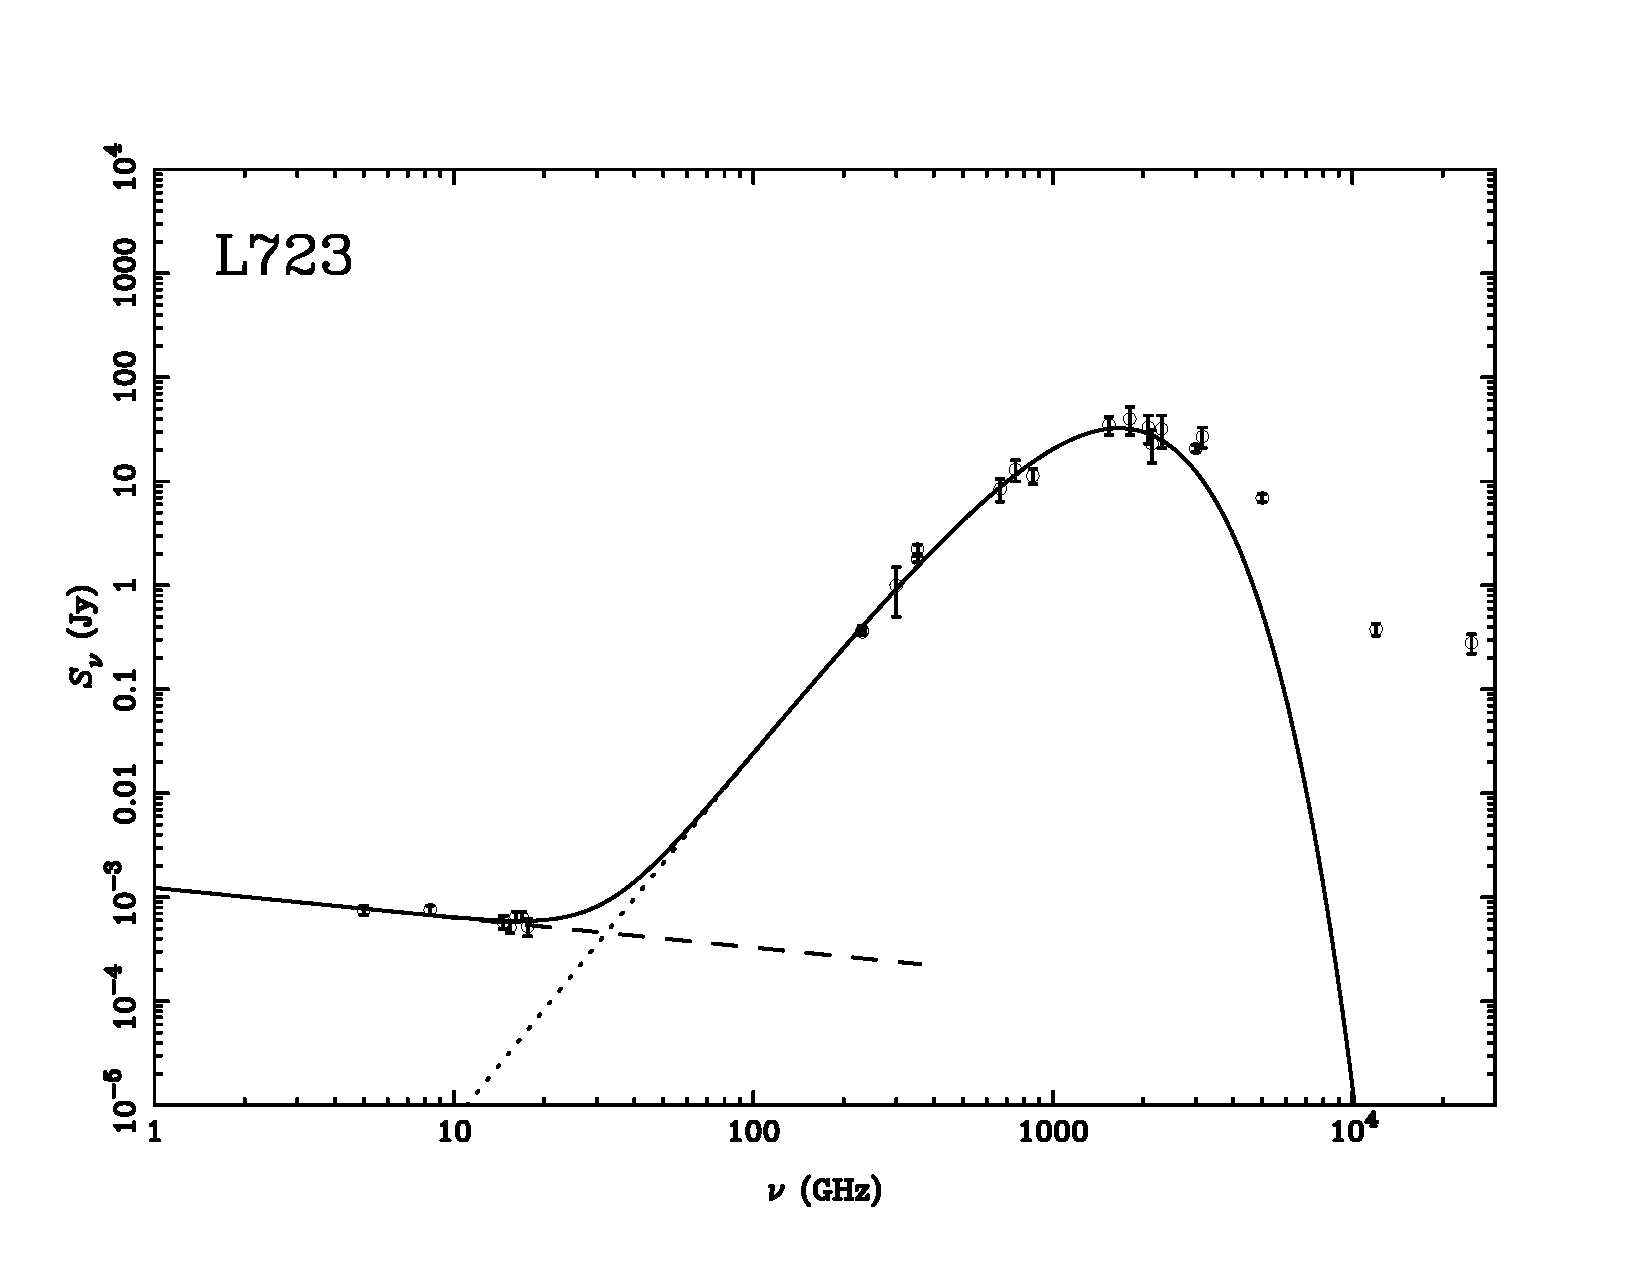
\includegraphics[width=0.65\textwidth]{plots/L723.pdf}
\label{default}
\end{center}
\end{figure}

\clearpage



%%%%%
\begin{table}
\caption{L$1251$~A}
\begin{center}
\begin{tabular}{llll}
\hline
 & $\nu$ & $S_\nu$ & Reference\\
 & (GHz) & (Jy) & \\
\hline
 & $5$ & $(1.7\pm0.03)\times10^{-4}$ & \citet{2001AJ....121.1556B}\\
 & $8$ & $2.9\times10^{-4\dag}$ & \citet{2004AJ...127.1736R}\\
 & $8$ & $(4.7\pm0.03)\times10^{-4}$ & \citet{2001AJ....121.1556B}\\
 & $14.62$ & $(8.57\pm1.77)\times10^{-4}$ & \citet{2012MNRAS.423.1089A}\\
 & $15.37$ & $(9.85\pm1.36)\times10^{-4}$ & \citet{2012MNRAS.423.1089A}\\
 & $16.12$ & $(1.00\pm0.20)\times10^{-3}$ & \citet{2012MNRAS.423.1089A}\\
 & $16.87$ & $(7.61\pm1.58)\times10^{-4}$ & \citet{2012MNRAS.423.1089A}\\
 & $17.62$ & $(1.10\pm0.23)\times10^{-3}$ & \citet{2012MNRAS.423.1089A}\\
 & $230$ & $0.23\pm0.02$ & \citet{1995PASP..107...49R}\\
 & $273$ & $0.38\pm0.03$ & \citet{1995PASP..107...49R}\\
 & $353$ & $5.68^{\dag}$ & \citet{2008ApJS..175..277D}\\
 & $375$ & $0.71\pm0.11$ & \citet{1995PASP..107...49R}\\
 & $857$ & $20.8\pm3.2$ & \citet{2007AJ....133.1560W}\\
 & $3\times10^{3}$ & $78.5\pm12.6$ & \citet{1995PASP..107...49R}\\
 & $3\times10^{3}$ & $79^{\dag}$ & \citet{1989ApJ...343..773S}\\
 & $5\times10^{3}$ & $67.7\pm6.1$ & \citet{1995PASP..107...49R}\\
 & $5\times10^{3}$ & $66^{\dag}$ & \citet{1989ApJ...343..773S}\\
 & $1.2\times10^{4}$ & $28.3\pm1.4$ & \citet{1995PASP..107...49R}\\
 & $1.2\times10^{4}$ & $26^{\dag}$ & \citet{1989ApJ...343..773S}\\
 & $2.5\times10^{4}$ & $6.2\pm0.3$ & \citet{1995PASP..107...49R}\\
 & $2.5\times10^{4}$ & $5^{\dag}$ & \citet{1989ApJ...343..773S}\\
\end{tabular}
\end{center}
\label{default}
\end{table}%

\begin{figure}[htbp]
\begin{center}
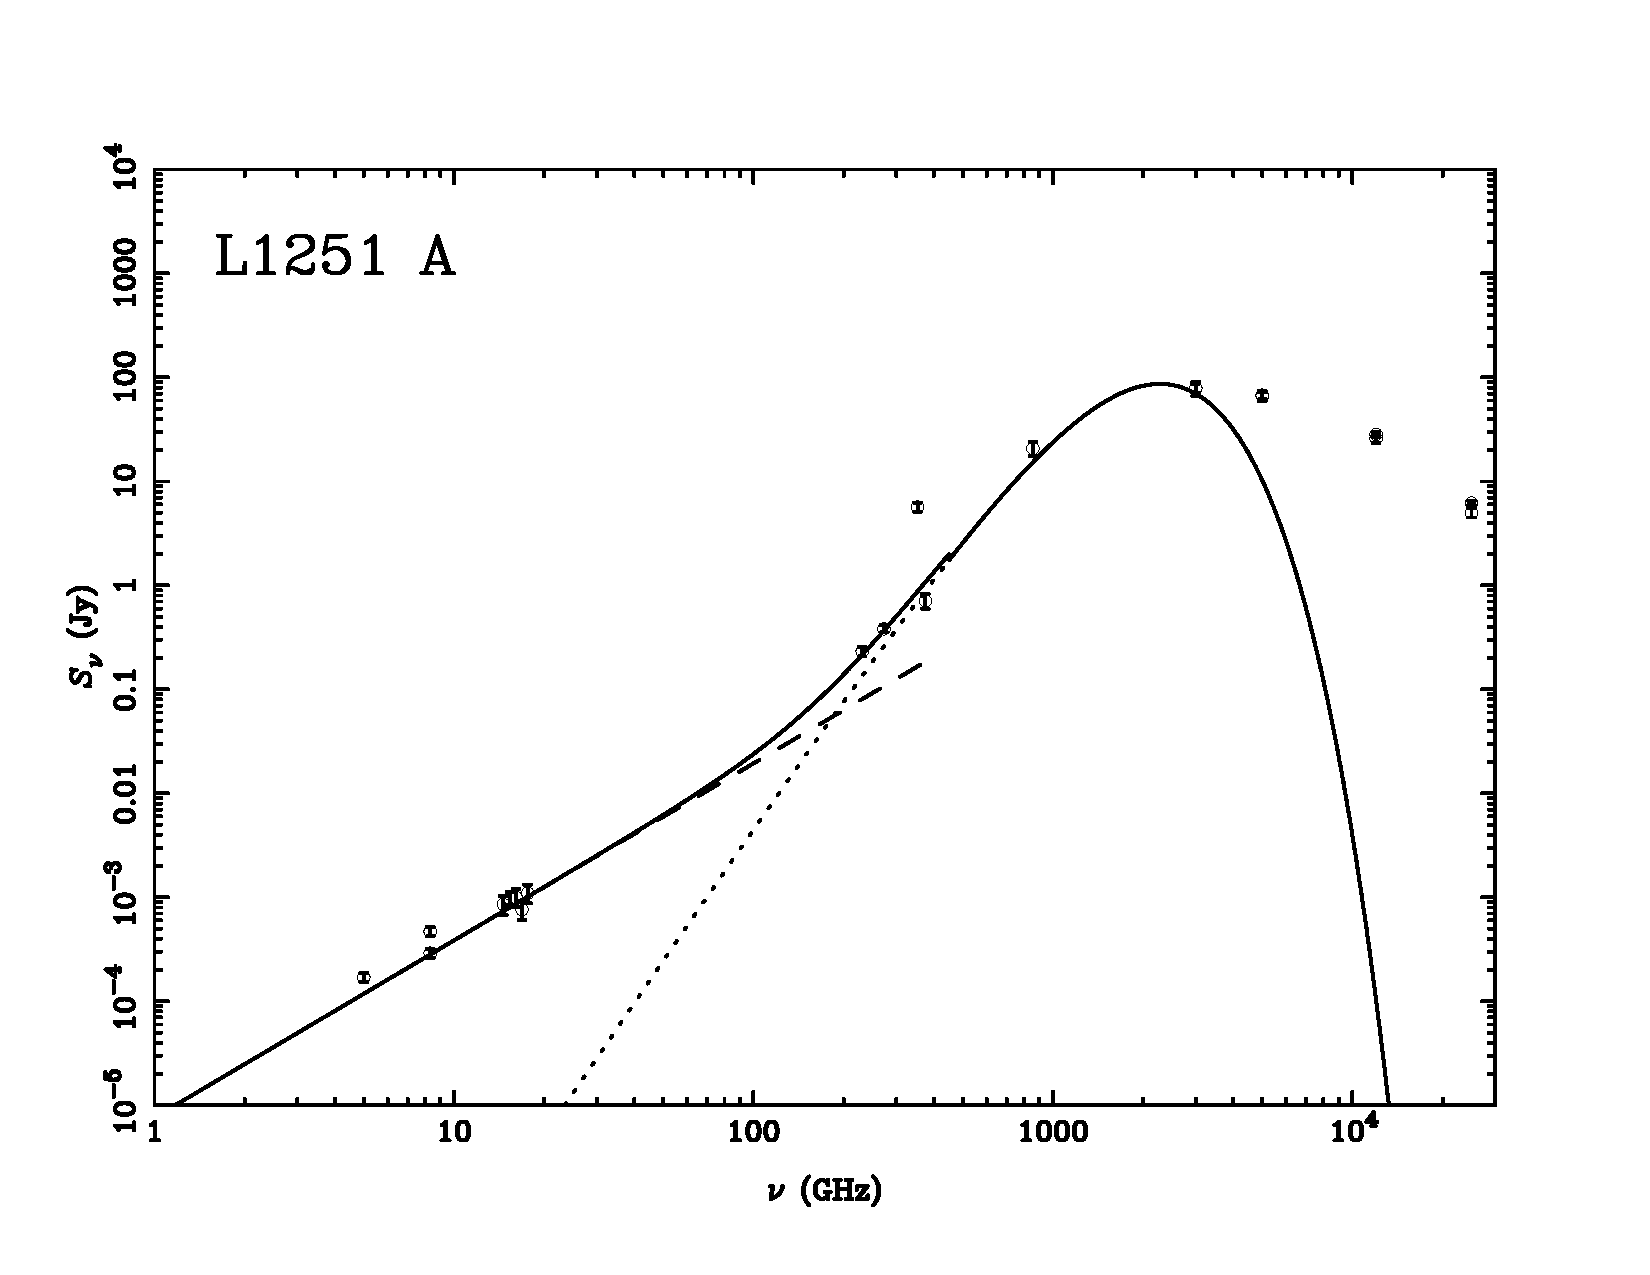
\includegraphics[width=0.65\textwidth]{plots/L1251.pdf}
\label{default}
\end{center}
\end{figure}

\clearpage



%%%%%
\begin{table}
\caption{L$1448$~C}
\begin{center}
\begin{tabular}{llll}
\hline
 & $\nu$ & $S_\nu$ & Reference\\
 & (GHz) & (Jy) & \\
\hline
 & $8$ & $2.3\times10^{-4\dag}$ & \citet{2002AJ....124.1045R}\\
 & $15$ & $(5.6\pm0.5)\times10^{-4}$ & \citet{1990ApJ...365L..85C}\\
 & $16$ & $(5.37\pm0.33)\times10^{-4}$ & \citet{2011MNRAS.415..893A}\\
 & $16.12$ & $(7.58\pm0.94)\times10^{-4}$ & \citet{2012MNRAS.423.1089A}\\
 & $86$ & $(2.6\pm0.2)\times10^{-2}$ & \citet{2000ApJS..131..249S}\\
 & $87$ & $1.2\times10^{-2\dag}$ & \citet{1991AA...241L..43B}\\
 & $87$ & $1.6\times10^{-2\dag}$ & \citet{1992AA...265L..49G}\\
 & $91$ & $(3.92\pm0.39)\times10^{-2}$ & \citet{2011AJ....141...39S}\\
 & $115$ & $(9.1\pm0.2)\times10^{-2}$ & \citet{2000ApJS..131..249S}\\
 & $230$ & $1\pm0.1$ & \citet{1998ApJ...509..733B}\\
 & $230$ & $0.74\pm0.11$ & \citet{2000ApJS..131..249S}\\
 & $230$ & $0.91^{\dag}$ & \citet{2001AA...365..440M}\\
 & $230$ & $0.58^{\dag}$ & \citet{1991AA...241L..43B}\\
 & $273$ & $2.04^{\dag}$ & \citet{2006ApJ...638..293E}\\
 & $273$ & $1\pm0.1$ & \citet{1998ApJ...509..733B}\\
 & $349$ & $1.97\pm0.13$ & \citet{2011AJ....141...39S}\\
 & $353$ & $2.98^{\dag}$ & \citet{2008ApJS..175..277D}\\
 & $353$ & $6.51^{\dag}$ & \citet{2007AA...468.1009H}\\
 & $353$ & $3.95\pm0.24$ & \citet{2000ApJS..131..249S}\\
 & $353$ & $5.34\pm0.43$ & \citet{2000ApJ...530..851C}\\
 & $375$ & $3\pm0.3$ & \citet{1998ApJ...509..733B}\\
 & $400$ & $6.91\pm0.91$ & \citet{2000ApJ...530..851C}\\
 & $666$ & $68.4^{\dag}$ & \citet{2007AA...468.1009H}\\
 & $666$ & $21\pm2$ & \citet{1998ApJ...509..733B}\\
 & $666$ & $31.8\pm5.5$ & \citet{2000ApJS..131..249S}\\
 & $666$ & $34.2\pm6.9$ & \citet{2000ApJ...530..851C}\\
 & $857$ & $58\pm18$ & \citet{2000ApJ...530..851C}\\
 & $857$ & $30\pm3$ & \citet{1998ApJ...509..733B}\\
 & $3\times10^{3}$ & $70.3\pm14.8$ & \citet{1998ApJ...509..733B}\\
 & $5\times10^{3}$ & $31.2\pm6.5$ & \citet{1998ApJ...509..733B}\\
 & $1.2\times10^{4}$ & $2.9\pm0.6$ & \citet{1998ApJ...509..733B}\\
 & $2.5\times10^{4}$ & $0.33\pm0.07$ & \citet{1998ApJ...509..733B}\\
\end{tabular}
\end{center}
\label{default}
\end{table}%

\begin{figure}[htbp]
\begin{center}
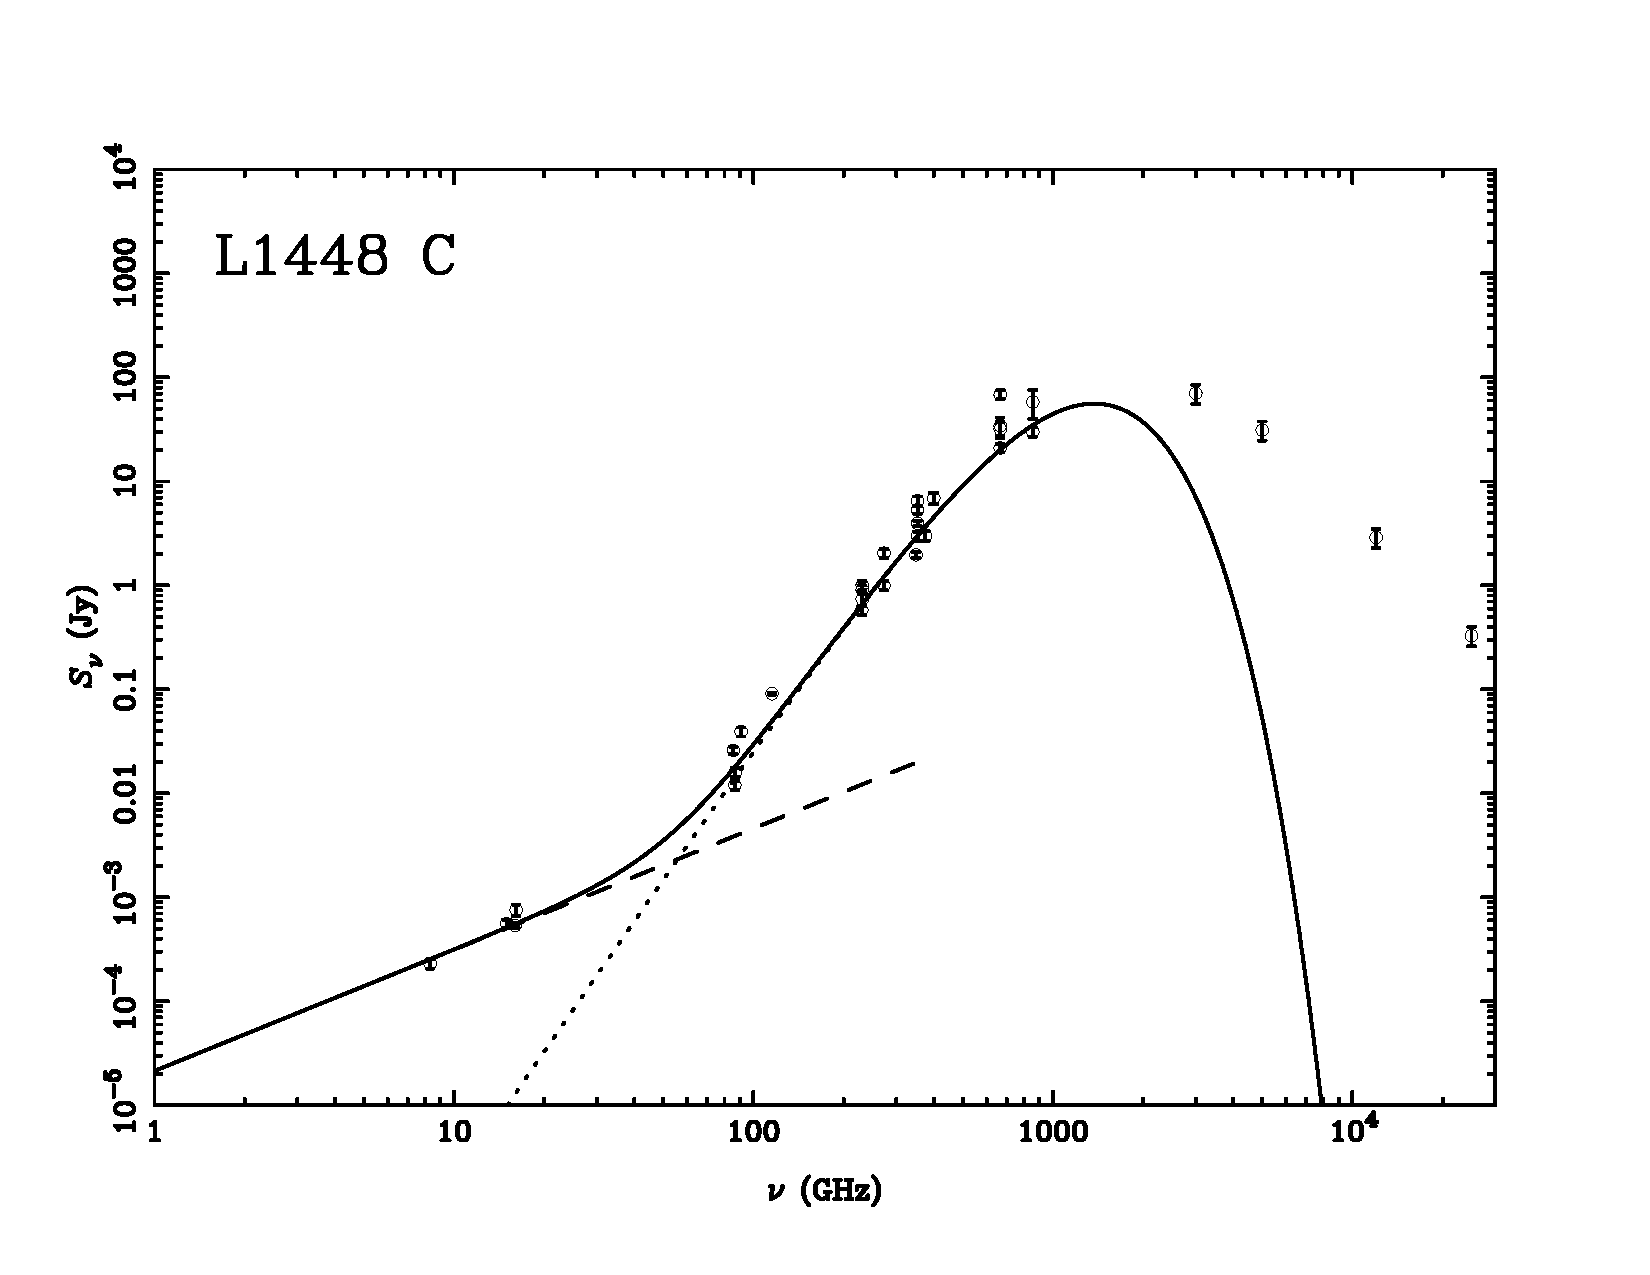
\includegraphics[width=0.65\textwidth]{plots/L1448C.pdf}
\label{default}
\end{center}
\end{figure}

\clearpage



%%%%%
\begin{table}
\caption{NGC~$1333$~\textit{IRAS}~$2$A}
\begin{center}
\begin{tabular}{llll}
\hline
 & $\nu$ & $S_\nu$ & Reference\\
 & (GHz) & (Jy) & \\
\hline
 & $5$ & $(6\pm1)\times10^{-5}$ & \citet{1999ApJS..125..427R}\\
 & $8$ & $2.2\times10^{-4\dag}$ & \citet{2002AJ....124.1045R}\\
 & $8$ & $(2.5\pm0.4)\times10^{-4}$ & \citet{1999ApJS..125..427R}\\
 & $16$ & $(3.2\pm0.25)\times10^{-4}$ & \citet{2011MNRAS.415..893A}\\
 & $16.12$ & $(3.92\pm0.96)\times10^{-4}$ & \citet{2012MNRAS.423.1089A}\\
 & $43$ & $(1\pm0.5)\times10^{-2}$ & \citet{2004ApJ...605L.137A}\\
 & $86$ & $3.5\times10^{-2\dag}$ & \citet{2004AA...413..993J}\\
 & $89$ & $4\times10^{-2\dag}$ & \citet{2004AA...413..993J}\\
 & $111$ & $(8.28\pm0.4)\times10^{-2}$ & \citet{2000ApJ...529..477L}\\
 & $150$ & $0.32\pm0.07$ & \citet{1994AA...285L...1S}\\
 & $230$ & $0.88^{\dag}$ & \citet{2001AA...365..440M}\\
 & $230$ & $0.88\pm0.12$ & \citet{1994AA...285L...1S}\\
 & $273$ & $1.46\pm0.12$ & \citet{1994AA...285L...1S}\\
 & $353$ & $7.78^{\dag}$ & \citet{2007ApJ...668.1042K}\\
 & $353$ & $4.79\pm0.39$ & \citet{2000ApJ...530..851C}\\
 & $375$ & $4.08\pm0.05$ & \citet{1994AA...285L...1S}\\
 & $375$ & $3.75\pm0.15$ & \citet{1994AA...285L...1S}\\
 & $400$ & $5.54\pm0.21$ & \citet{1994AA...285L...1S}\\
 & $400$ & $6.61\pm0.86$ & \citet{2000ApJ...530..851C}\\
 & $666$ & $43\pm11$ & \citet{2000ApJ...530..851C}\\
 & $666$ & $23.7\pm0.9$ & \citet{1994AA...285L...1S}\\
 & $857$ & $37.2\pm1.2$ & \citet{1994AA...285L...1S}\\
 & $857$ & $74\pm22$ & \citet{2000ApJ...530..851C}\\
 & $3\times10^{3}$ & $300^{\dag}$ & \citet{1987MNRAS.226..461J}\\
 & $6\times10^{3}$ & $104^{\dag}$ & \citet{1987MNRAS.226..461J}\\
\end{tabular}
\end{center}
\label{default}
\end{table}%

\begin{figure}[htbp]
\begin{center}
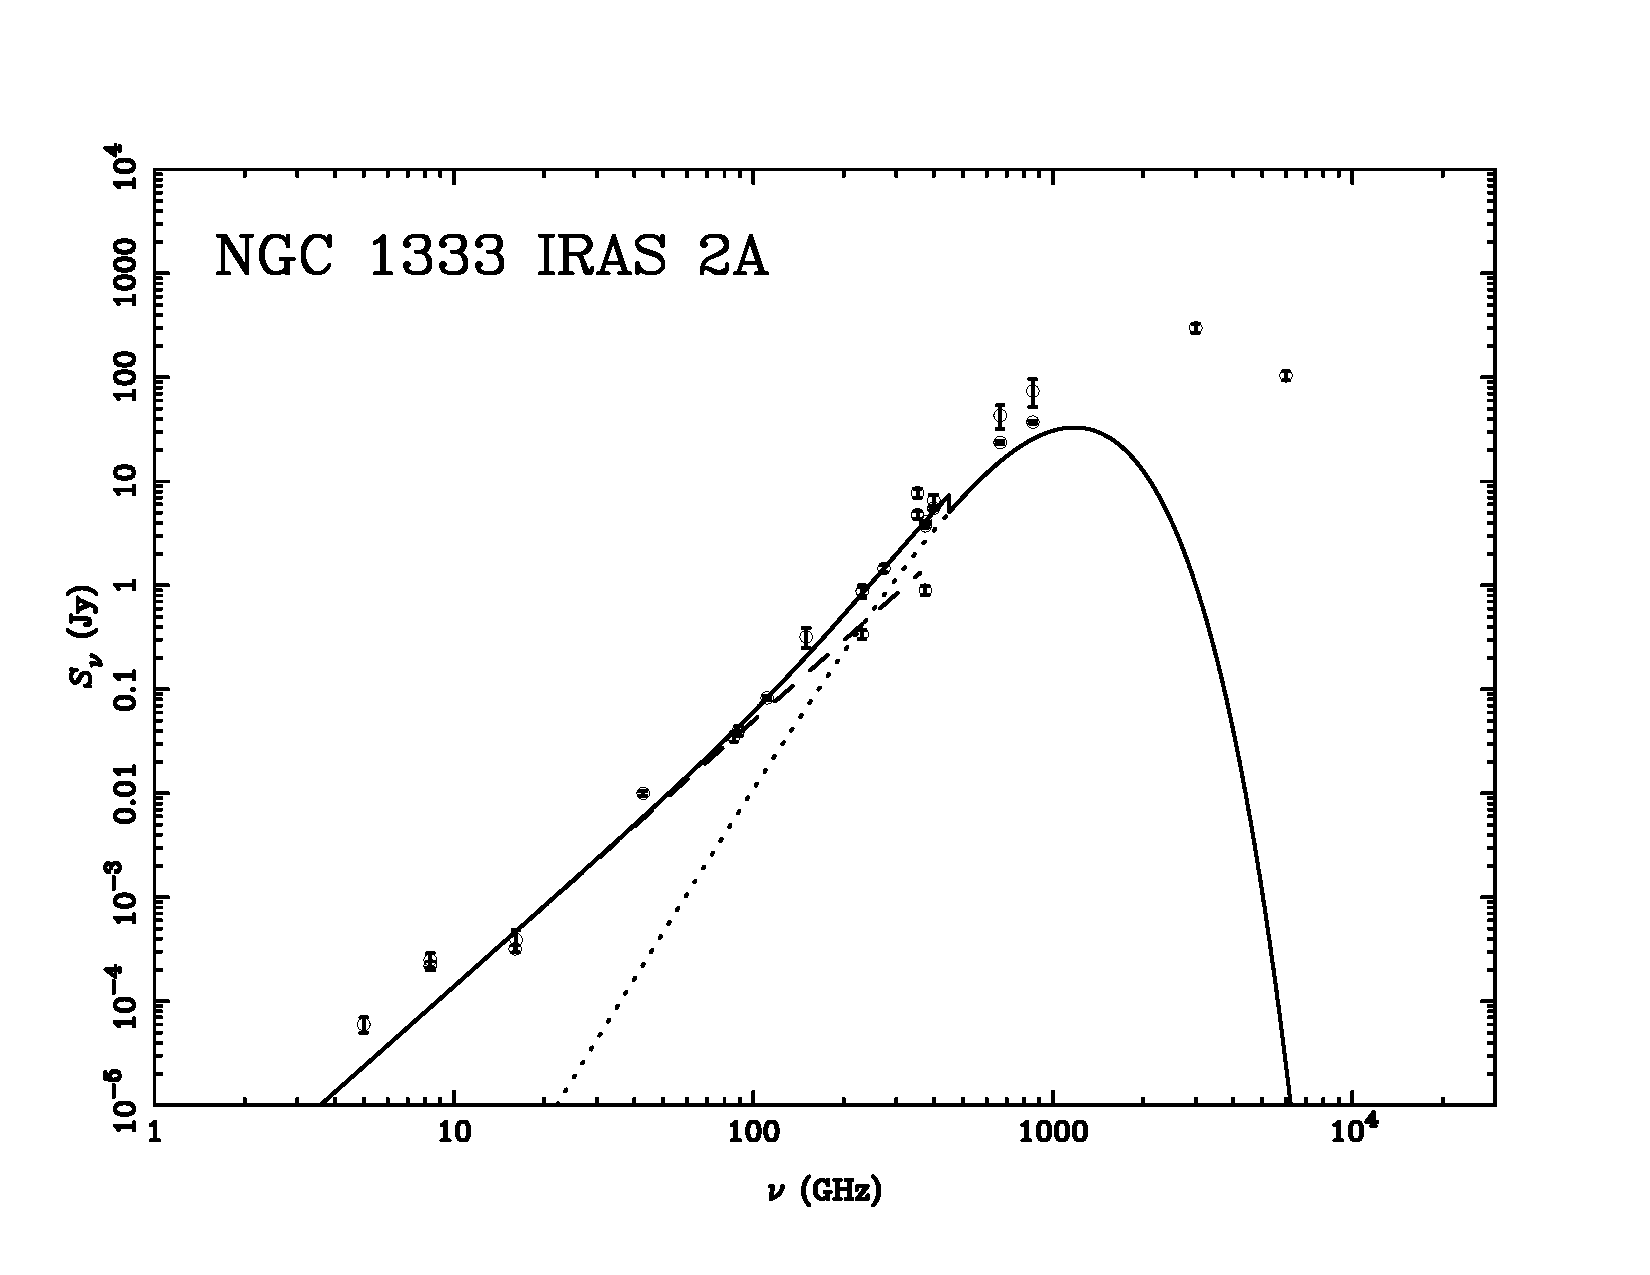
\includegraphics[width=0.65\textwidth]{plots/HH7-11-IRAS2A.pdf}
\label{default}
\end{center}
\end{figure}

\clearpage



%%%%%
\begin{table}
\caption{NGC~$1333$~\textit{IRAS}~$2$B}
\begin{center}
\begin{tabular}{llll}
\hline
 & $\nu$ & $S_\nu$ & Reference\\
 & (GHz) & (Jy) & \\
\hline
 & $5$ & $(2.3\pm0.1)\times10^{-4}$ & \citet{1999ApJS..125..427R}\\
 & $8$ & $(4\pm0.2)\times10^{-4}$ & \citet{1999ApJS..125..427R}\\
 & $8$ & $(3.7\pm0.37)\times10^{-4}$ & \citet{2002AJ....124.1045R}\\
 & $16$ & $(1.21\pm0.05)\times10^{-3}$ & \citet{2011MNRAS.415..893A}\\
 & $16.12$ & $(5.05\pm1.01)\times10^{-4}$ & \citet{2012MNRAS.423.1089A}\\
 & $43$ & $(5.2\pm0.3)\times10^{-3}$ & \citet{2004ApJ...605L.137A}\\
 & $86$ & $1.2\times10^{-2\dag}$ & \citet{2004AA...413..993J}\\
 & $89$ & $1.4\times10^{-2\dag}$ & \citet{2004AA...413..993J}\\
 & $111$ & $(2.77\pm0.32)\times10^{-2}$ & \citet{2000ApJ...529..477L}\\
 & $353$ & $1.19\pm0.1$ & \citet{2000ApJ...530..851C}\\
 & $400$ & $1.53\pm0.21$ & \citet{2000ApJ...530..851C}\\
 & $666$ & $7.7\pm1.6$ & \citet{2000ApJ...530..851C}\\
 & $857$ & $13.4\pm1.3$ & \citet{2000ApJ...530..851C}\\
\end{tabular}
\end{center}
\label{default}
\end{table}%

\begin{figure}[htbp]
\begin{center}
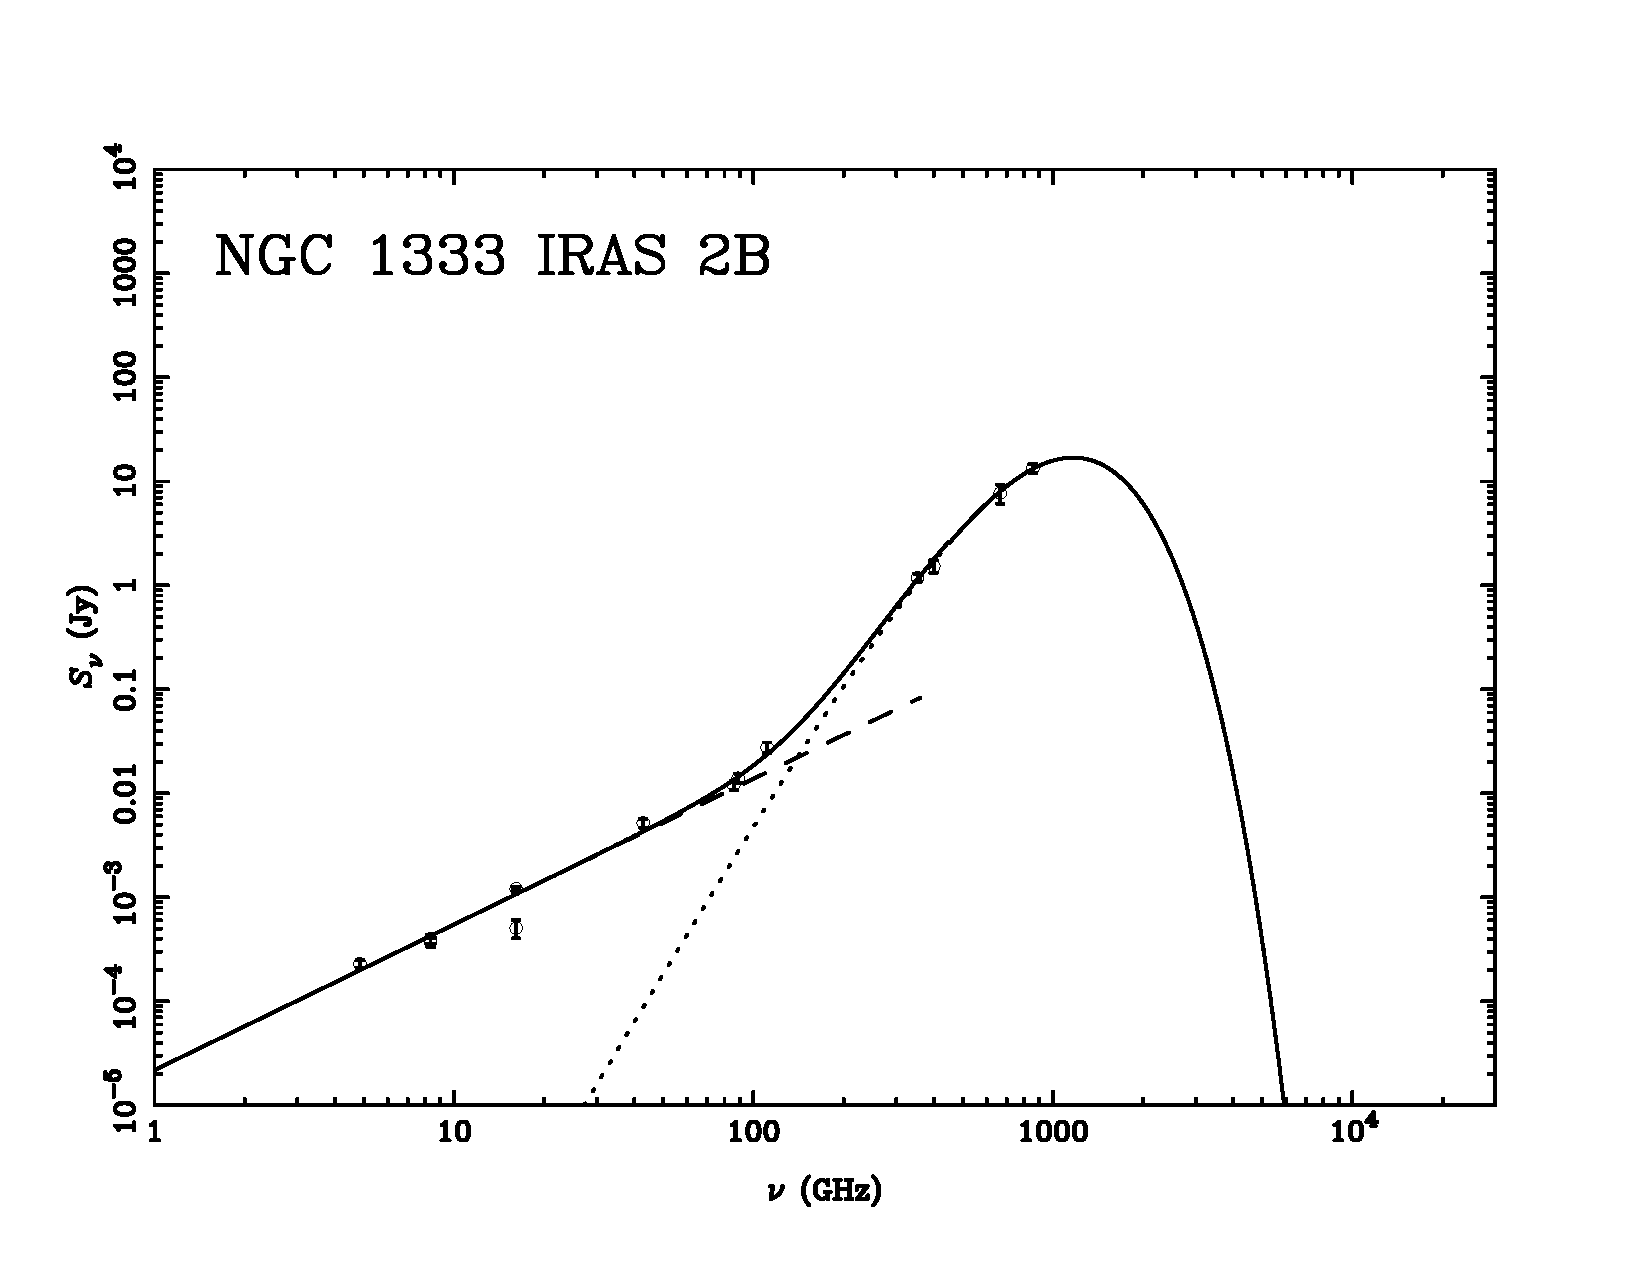
\includegraphics[width=0.65\textwidth]{plots/HH7-11-IRAS2B.pdf}
\label{default}
\end{center}
\end{figure}

\clearpage



%%%%%
\begin{table}
\caption{L$1551$~NE}
\begin{center}
\begin{tabular}{llll}
\hline
 & $\nu$ & $S_\nu$ & Reference\\
 & (GHz) & (Jy) & \\
\hline
 & $8$ & $6.6\times10^{-4\dag}$ & \citet{2002AJ....124.1045R}\\
 & $16.12$ & $(7.43\pm0.92)\times10^{-4}$ & \citet{2012MNRAS.423.1089A}\\
 & $230$ & $1.5^{\dag}$ & \citet{2001AA...365..440M}\\
 & $230$ & $0.85\pm0.01$ & \citet{2005ApJ...631.1134A}\\
 & $230$ & $0.85\pm0.08$ & \citet{2000ApJ...533L.143M}\\
 & $238$ & $0.8\pm0.12$ & \citet{1993ApJ...406L..71B}\\
 & $272$ & $1.07\pm0.11$ & \citet{1993ApJ...406L..71B}\\
 & $353$ & $2.78^{\dag}$ & \citet{2006ApJ...645..357M}\\
 & $353$ & $10.5^{\dag}$ & \citet{2008ApJS..175..277D}\\
 & $379$ & $2.22\pm0.37$ & \citet{1993ApJ...406L..71B}\\
 & $666$ & $8.33^{\dag}$ & \citet{2006ApJ...645..357M}\\
 & $677$ & $16.2\pm4.6$ & \citet{1993ApJ...406L..71B}\\
 & $857$ & $22.83\pm0.72$ & \citet{2005ApJ...631.1134A}\\
 & $3\times10^{3}$ & $130^{\dag}$ & \citet{1984ApJ...278L..49E}\\
 & $5\times10^{3}$ & $80^{\dag}$ & \citet{1984ApJ...278L..49E}\\
 & $1.2\times10^{4}$ & $16^{\dag}$ & \citet{1984ApJ...278L..49E}\\
 & $2.5\times10^{4}$ & $1.2^{\dag}$ & \citet{1984ApJ...278L..49E}\\
\end{tabular}
\end{center}
\label{default}
\end{table}%


\begin{figure}[htbp]
\begin{center}
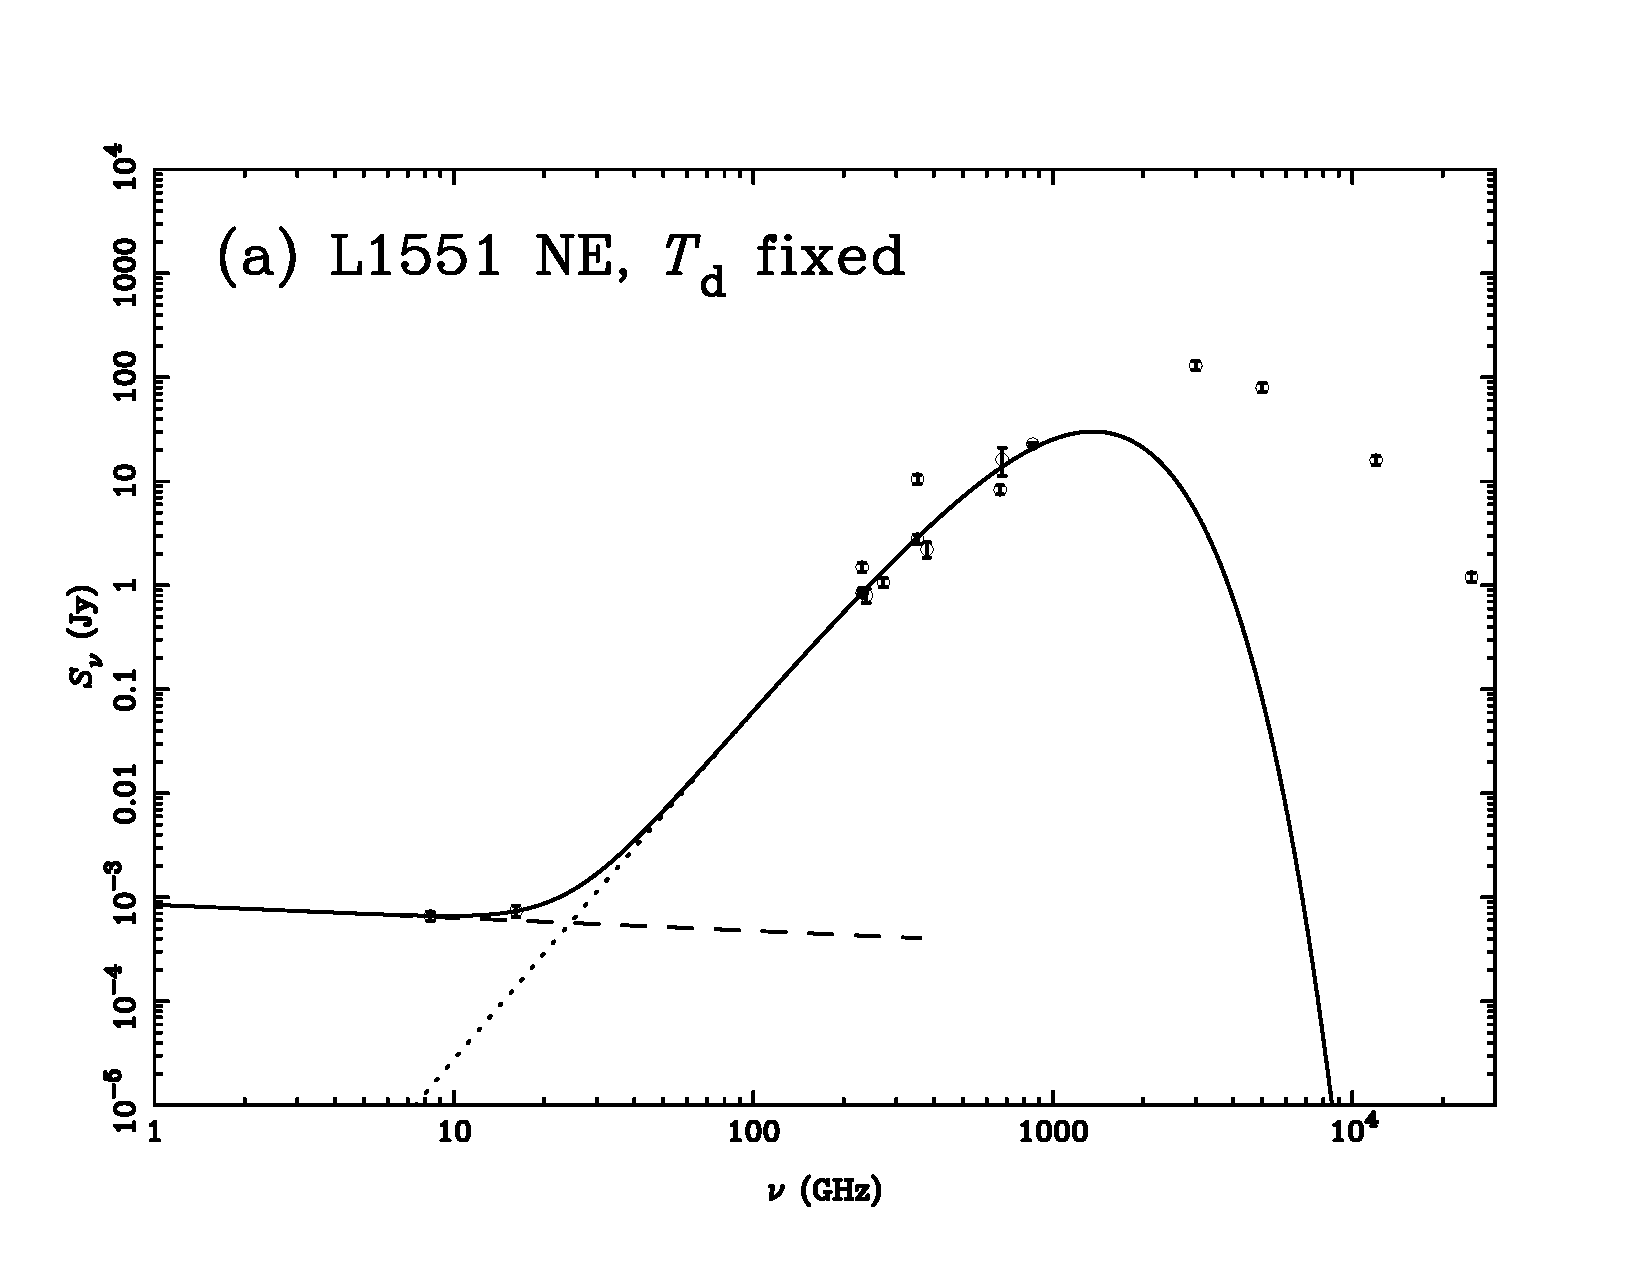
\includegraphics[width=0.65\textwidth]{plots/L1551NE-TdFixed.pdf}\\
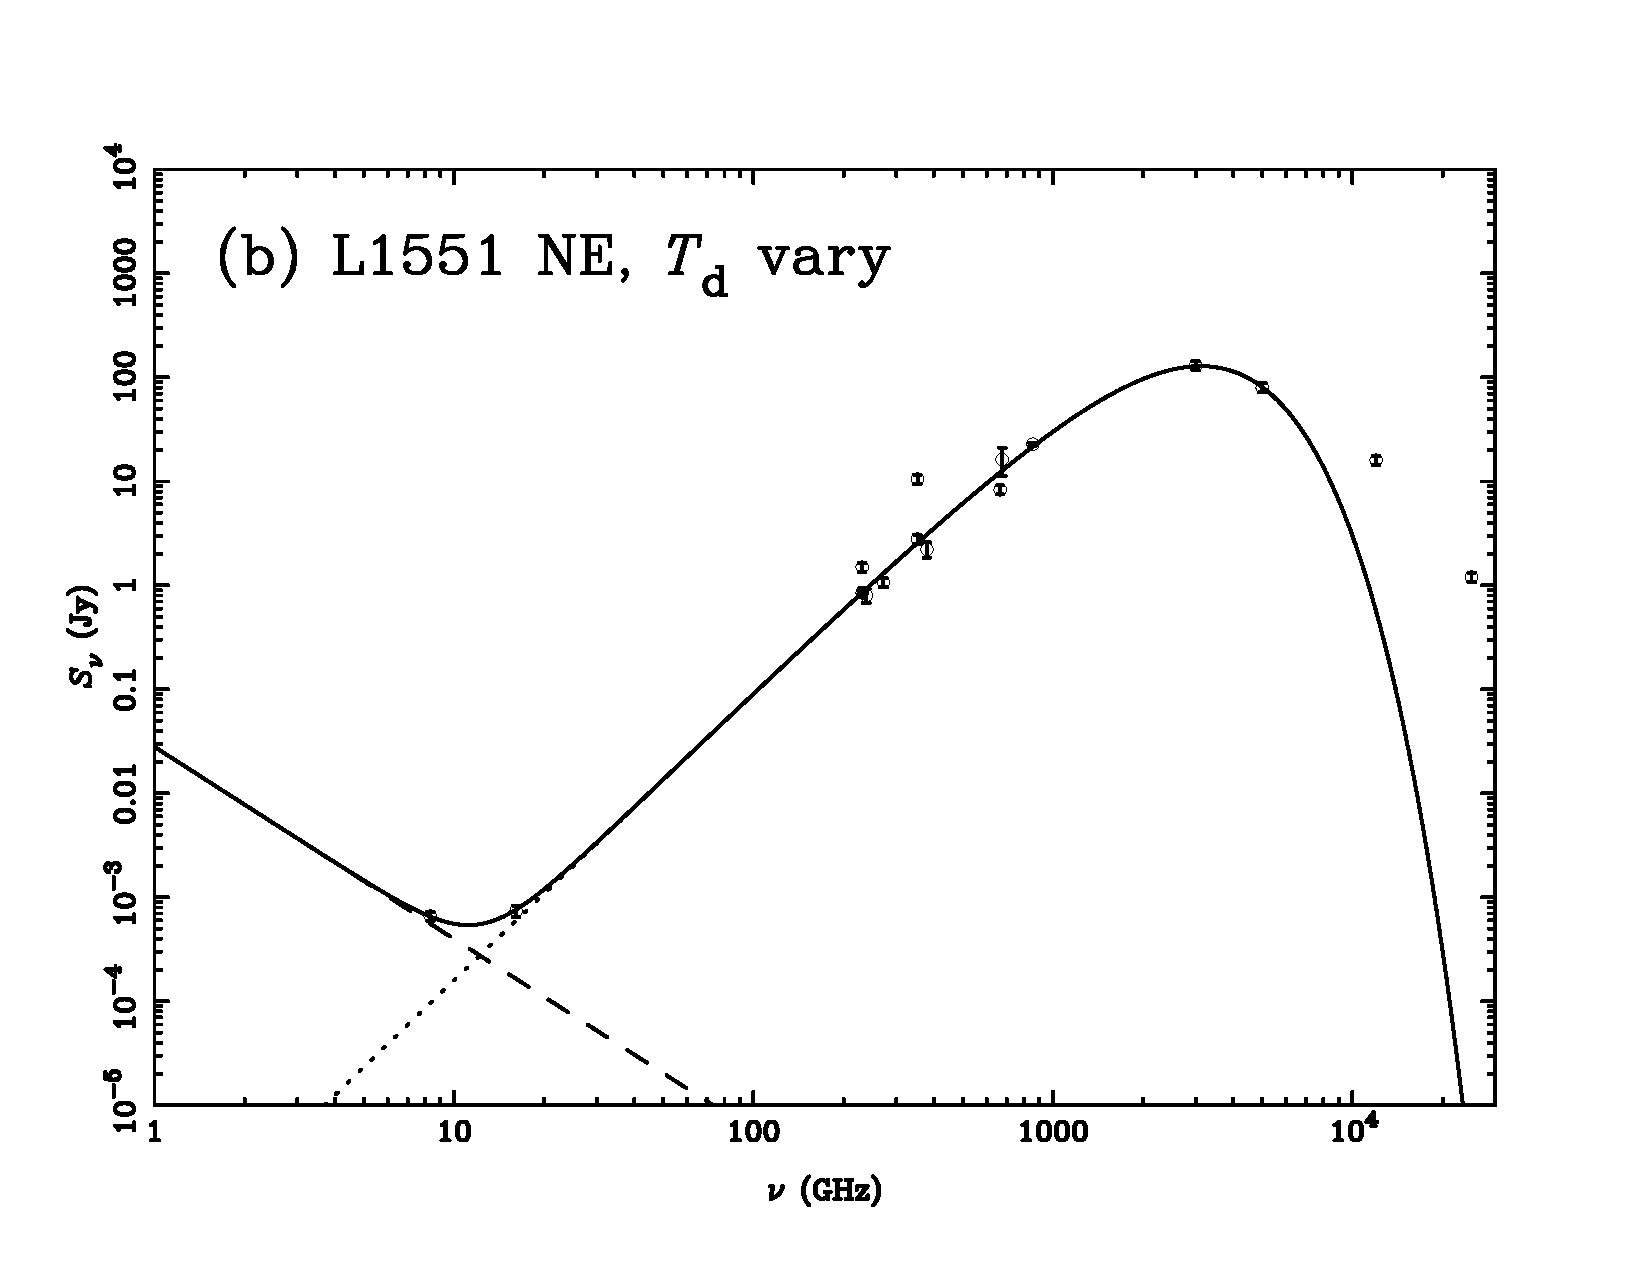
\includegraphics[width=0.65\textwidth]{plots/L1551NE.pdf}
\label{default}
\end{center}
\end{figure}

\clearpage



%%%%%
\begin{table}
\caption{HH~$25$~MMS}
\begin{center}
\begin{tabular}{llll}
\hline
 & $\nu$ & $S_\nu$ & Reference\\
 & (GHz) & (Jy) & \\
\hline
 & $5$ & $(1.5\pm0.4)\times10^{-4}$ & \citet{1995AA...297...98B}\\
 & $8$ & $(2.5\pm0.6)\times10^{-4}$ & \citet{1995AA...297...98B}\\
 & $8$ & $(1.6\pm0.3)\times10^{-4}$ & \citet{1999MNRAS.304....1G}\\
 & $16.12$ & $(1.23\pm0.10)\times10^{-3}$ & \citet{2012MNRAS.423.1089A}\\
 & $231$ & $1^{\dag}$ & \citet{1999ApJ...527..856L}\\
 & $353$ & $9.11^{\dag}$ & \citet{2008ApJS..175..277D}\\
 & $353$ & $4^{\dag}$ & \citet{2007MNRAS.374.1413N}\\
 & $666$ & $10.8^{\dag}$ & \citet{2007MNRAS.374.1413N}\\
 & $666$ & $8.7^{\dag}$ & \citet{2001MNRAS.326..927P}\\
 & $353$ & $1.4^{\dag}$ & \citet{2001MNRAS.326..927P}\\
 & $857$ & $24^{\dag}$ & \citet{1999ApJ...527..856L}\\
 & $3\times10^{3}$ & $70.66^{\dag}$ & \textit{IRAS}\\
 & $5\times10^{3}$ & $28.04^{\dag}$ & \textit{IRAS}\\
 & $5\times10^{3}$ & $32^{\dag}$ & \textit{IRAS}\\
 & $1.2\times10^{4}$ & $1.39^{\dag}$ & \citet{1999yCat.2225....0G}\\
 & $2.5\times10^{4}$ & $0.51^{\dag}$ & \citet{1999yCat.2225....0G}\\
\end{tabular}
\end{center}
\label{default}
\end{table}%


\begin{figure}[htbp]
\begin{center}
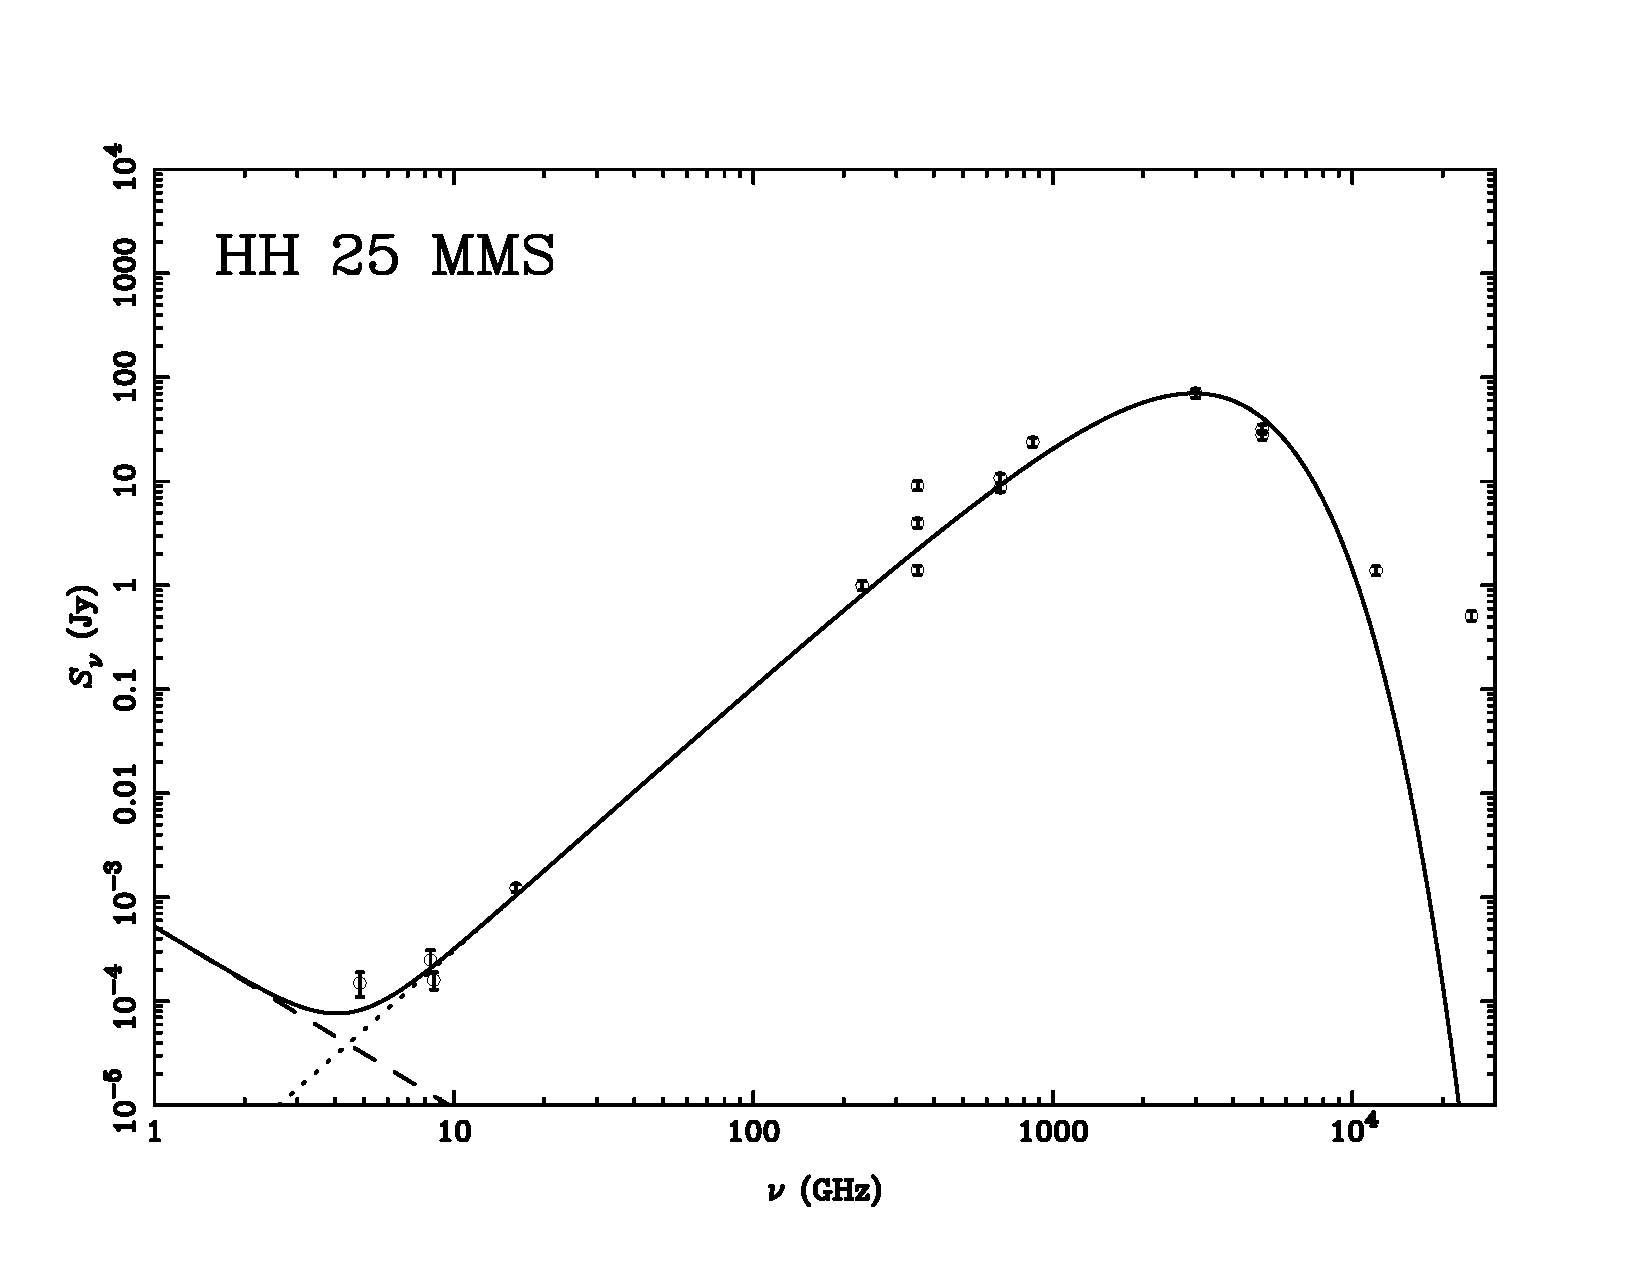
\includegraphics[width=0.65\textwidth]{plots/HH25MMS.pdf}
\label{default}
\end{center}
\end{figure}


\clearpage
%%%%%%%%%%%%%%%%%%%% REFERENCES %%%%%%%%%%%%%%%%%%


\bibliographystyle{apj}
\bibliography{Bibliography} % if your bibtex file is called Bibliography.bib


\end{document}  